%!TEX program = lualatex 
%!TEX encoding = UTF-8 Unicode  
%!TEX root = chapter06.tex  
\documentclass[main.tex]{subfiles} 
\begin{document} 
%----------------------------------------------------------------------------------------
%	CHAPTER 6
%----------------------------------------------------------------------------------------
\newpage 
\loadgeometry{marginlayout}  
\pagestyle{scrheadings} % Print headers again  
\KOMAoptions{
headwidth=textwithmarginpar,
headsepline=true,
headsepline= 0.5pt,
footwidth=textwithmarginpar,
}  
\onehalfspacing 
\setcounter{chapter}{5}

\chapter{La fonction exponentielle}  
\section{Définition et propriétés}

\begin{theorem}\label{chapter06:theorem:existence} Il existe une fonction dérivable sur $\mathbb{R}$ tel que $f(0)=1$ et $f'=f$.
\end{theorem}
\begin{proposition} Une telle fonction ne s'annulle pas.	
\end{proposition}
\begin{proof} On définit la fonction $\varphi$ sur $\mathbb{R}$ par $\varphi(x)=f(x)f(-x)$.\\
$\begin{WithArrows}
	\varphi'(x)& = f'(x)f(-x)+ f(x)\times (-f'(-x))\\
	& = f(x)f(-x)-f(x)f(-x)\\
	&=0
	\end{WithArrows}$ et 
$\begin{WithArrows}
	\varphi(0)& = f(0)f(-0)=1
\end{WithArrows}$. 

$\varphi$ est de dérivée nulle sur $\mathbb{R}$, c'est une fonction constante, et pour tout $x\in \mathbb{R}$ : $f(x)f(-x)=\varphi(x)=1$.

En conséquence $f(x)\neq 0$.
\end{proof}
\begin{proposition}\label{chapter06:proposition:unicite}  Une telle fonction est unique.	
\end{proposition}
\begin{proof} Prenons deux fonctions $f$ et $g$ vérifiant le théorème \ref{chapter06:theorem:existence}. On définit la fonction $\psi$ sur $\mathbb{R}$ par :
	\setlength{\abovedisplayskip}{3pt}
	\setlength{\belowdisplayskip}{3pt}
	$$\psi(x)=\frac{f(x)}{g(x)}$$
$\begin{WithArrows}
	\psi'(x)& = \frac{f'(x)g(x)-f(x)g'(x)}{g^2(x)} \\
	& =  \frac{f(x)g(x)-f(x)g(x)}{g^2(x)} \\
	&= 0 
\end{WithArrows}$ et 
$\begin{WithArrows}
	\psi(0)& = \frac{f(0)}{g(0)}=1
\end{WithArrows}$.
	
	$\psi$ est de dérivée nulle sur $\mathbb{R}$, c'est une fonction constante, et pour tout $x\in \mathbb{R}$ : $\frac{f(x)}{g(x)}=\psi(x)=1$ et $f(x)=g(x)$.
\end{proof}
\begin{definition}[notation 1] On note \og $\exp$ \fg l'unique fonction dérivable sur $\mathbb{R}$ vérifiant $f'=f$ et $f(0)=1$.
\end{definition}
\begin{definition}[nombre d'Euler] On note $e=\exp(1)\approx $ \pyc{print(round(numpy.e,8))}.
\end{definition}
\begin{properties}Pour tout $x$ et $y\in\mathbb{R}$ et $n\in\mathbb{N}$
	\begin{enumerate}[label=(\roman*),leftmargin=*]
		\item $\exp(0)=1$
		\item $\exp(-x)=\frac{1}{\exp(x)}$
		\item\label{chapter06:properties:produit}  $\exp(x+y)=\exp(x)\exp(y)$.\\
		\null\hfill  En particulier $\exp(x+1)=e\exp(x)$
		\item $\exp(nx)=\big(\exp(x)\big)^n$.\\
		\null\hfill  En particulier $\exp(2x)=(\exp(x))^2$.
		\item $\exp(x)>0$, et $\sqrt{\exp(x)}=\exp\left(\frac{x}{2}\right)$.
	\end{enumerate}
\end{properties}
\begin{proof}\hfill 
	\begin{enumerate}[label=(\roman*),leftmargin=*]
		\item par définition
		\item vu dans la démonstration de la proposition \ref{chapter06:proposition:unicite}
		\item Pour $y$ fixé, on définit la fonction $\gamma$ sur $\mathbb{R}$ par  $\gamma(x)=\frac{\exp(x+y)}{\exp(y)}$.\\
		$\begin{WithArrows}
			\gamma'(x)& = \gamma(x)  
		\end{WithArrows}$ et 
		$\begin{WithArrows}
			\gamma(0)& = \frac{\exp(0+y)}{\exp(y)}=1
		\end{WithArrows}$.\\
		$\gamma$ vérifie aussi les conditions du théorème \ref{chapter06:theorem:existence}. \\
		Par unicité on a $\gamma=\exp$.
		\item conséquence directe de \ref{chapter06:properties:produit}  
		\item $\exp(x)=\exp\left(\frac{x}{2}+\frac{x}{2}\right)= \exp\left(\frac{x}{2}\right)\exp\left(\frac{x}{2}\right)=\left(\exp\left(\frac{x}{2}\right)\right)^2$.
	\end{enumerate}
\end{proof}
\begin{definition}[notation 2] On note pour tout $x\in\mathbb{R}$ : $\eu^x=\exp(x)$.	 
\end{definition}
Cette notation est cohérente avec le fait que la fonction exponentielle hérite des propriétés connues des puissances :\medskip
\begin{enumerate}[label=\textbullet]
	\item  $\eu^0=1$ ; \qquad  $e=\eu^1$ et $\sqrt{e}=\eu^{\tfrac{1}{2}}$\medskip
	\item $\eu^{-x}=\frac{1}{\eu^x}$ ~; \qquad  $\eu^{x+y}=\eu^x\eu^y$ \qquad et  $\eu^{x-y}=\frac{\eu^x}{\eu^y}$\medskip
	\item $(\eu^x)^n=\eu^{nx}$ pour $n\in\mathbb{N}$ 
\end{enumerate}
\begin{remark}
Pour un exposant $n\in\mathbb{N}$ on a : $\eu^n=e\times e\ldots e$ et $\eu^{-n}=\frac{1}{\eu^n}$
\end{remark}
\begin{remark}
La suite $\big(\eu^{nx}\big)=\big(\exp(nx)\big)_{n\in\mathbb{N}}$ est une suite géométrique.
\end{remark}
\begin{marginfigure}[-4cm]
	\begin{tikzpicture}[scale = 1]
		\tkzInit[xmin=-3.0,xmax=2.0,ymin=-1.0,ymax=5,xstep=1.0, ystep=1.0];
		%	\begin{scope}[dashed] 
			%		\tkzGrid(-3,-1)(2,5);  
			%		%	\tkzGrid[ sub,color=black,subcolor=gray,subxstep=0.5,subystep=0.5](-5,-4)(6,5);  
			%	\end{scope} 
		\tkzDrawX[above=5pt, label={$x$}, font=\small, line width=1.2pt] 
		\tkzDrawY[ label={$y$}, font=\small, line width=1.2pt]
		\tkzLabelX[orig=false,below=5pt,   font=\scriptsize, line width=1.2] 
		\tkzLabelY[orig=false,left=5pt,  font=\scriptsize, line width=1.2]   
		\tkzFct[domain = -5.0:6.0,  line width=1.2pt, color=blue]{ 
			( exp(\x)) 
		}; 
		%	\tkzFct[domain = -5.0:6.0,  line width=1.2pt, color=red]{ 
			%	( log(\x)) 
			%}; 
		\tkzFct[domain = -4.0:5.0,  line width=1.2pt, color=black,dashed]{ 
			( \x+1.0) 
		}; 
		\tkzSetUpPoint[size=3, fill=black]
		\tkzfctset{tan style/.style={->,>=latex, color=red, line width=1.2pt}} 
		\tkzDefPointByFct[with=a,ref=A]({1});  
		\tkzDefPointByFct[with=a,ref=B]({0}); 
		%	\tkzDefPointByFct[with=b,ref=C]({1});  
		%	\tkzDefPointByFct[with=b,ref=D]({2.778}); 
		%	\tkzDrawPoints(A,B,C,D)
		\tkzDrawPoints(A,B)
		\tkzPointShowCoord[ylabel={$e$}](A) 
		%		\tkzPointShowCoord(D)  
	\end{tikzpicture}
	\end{marginfigure}
\begin{theorem} La fonction $x\mapsto \eu^x$ est strictement croissante sur $\mathbb{R}$.
\end{theorem}
\begin{proof}  Sa dérivée étant elle-même et elle est positive !
\end{proof}
\begin{theorem} La fonction $f\colon x\mapsto \eu^{ax+b}$ est dérivable sur $\mathbb{R}$ et on a $f'(x)=a\eu^{ax+b}$.
\end{theorem}

%----------------------------------------------------------------------------------------
%
%----------------------------------------------------------------------------------------
\newpage 
\loadgeometry{widelayout}  
\pagestyle{scrheadings} % Print headers again  
\KOMAoptions{
	headwidth=textwithmarginpar,
	headsepline=true,
	headsepline= 0.5pt,
	footwidth=textwithmarginpar,
}  
\onehalfspacing 
\vspace{-2mm}
\subsection{TP \no 1 : introduction aux fonctions exponentielles}	
\noindent Compléter le tableau de valeur à l'aide de votre calculatrice et tracer la représentation graphique de la fonction $f\colon x \mapsto 2^x$.

%\renewcommand{\arraystretch}{1.5} 
%\begin{tabularx}{0.9\linewidth}{|c|*{8}{Y|}}
%	\hline
%	$x$&$-2$&$-1$& $0$&$1$&$2$&$3$&$4$&$5$\\ \hline
%	$f(x)=2^x$& & & & & &&& \\\hline
%\end{tabularx} \\
\noindent
\parbox{0.8\linewidth}{ 
\begin{tikzpicture}[xscale=1.9, yscale = 1]
	\tkzSetUpPoint[size=5, fill=black]
	\tkzfctset{tan style/.style={->,>=latex, color=red, line width=1.2pt}}  
	\tkzInit[xmin=-3.0,xmax=4.0,ymin=0.0,ymax=20,xstep=1, ystep=2.0];
	\begin{scope}[dashed]   
		\tkzGrid[  color=black,sub,  subxstep=0.5,subystep=1](-3,0)(4,20); 
		\tkzGrid(-3,0)(4,20); 
	\end{scope} 
	\tkzDrawX[above=5pt, label={$x$}, font=\small, line width=1.2pt] 
	\tkzDrawY[ label={$y$}, font=\small, line width=1.2pt]
	\tkzLabelX[ below=5pt,   font=\scriptsize, line width=1.2] 
	\tkzLabelY[orig=false,left=5pt,  font=\scriptsize, line width=1.2]   
%	\tkzFct[domain = -3.0:5.0,  line width=1.2pt, color=black]{ 
%		( 2**\x+0.0) 
%	};  
%	\foreach \i in {-2,-1,...,4}{ 
%		\tkzDefPointByFct[with=a,ref=A\i]({\i});
%		\tkzDrawPoints(A\i)
%	}  
	%	\tkzDefPointByFct[with=a,ref=B]({0}); 
	%	\tkzDefPointByFct[with=b,ref=C]({1});  
	%	\tkzDefPointByFct[with=b,ref=D]({2.778}); 
	%	\tkzDrawPoints(A,B,C,D)
	%	\tkzDrawPoints(A,B)
	%	\tkzPointShowCoord[ylabel={$e$}](A) 
	%		\tkzPointShowCoord(D)  
\end{tikzpicture}
}
%\hfill 
\parbox{0.18\linewidth}{ 
\renewcommand{\arraystretch}{1.4} 
\begin{tabularx}{1\linewidth}{|c|Y|}
	\hline
	$x$& $f(x)=2^x$ \\ \hline
	$-3$ & \\ \hline
	$-2$ & \\ \hline
	$-1$ & \\ \hline
	$0$ & \\ \hline
	$0.5$ & \\ \hline
	$1$ & \\ \hline
	$1.5$ & \\ \hline
	$2$ & \\ \hline
	$2.5$ & \\ \hline
	$3$ & \\ \hline
	$4$ & \\ \hline
\end{tabularx}
}



\noindent 
Tracer à main levée sur le même repère les représentations graphiques de $x\mapsto 3^x$, $x\mapsto 2^x$ et $x\mapsto 1.5^x$ :\\
\noindent
\parbox{1\linewidth}{ \centering
	\begin{tikzpicture}[scale = 1]
	\tkzSetUpPoint[size=5, fill=black]
	\tkzfctset{tan style/.style={->,>=latex, color=red, line width=1.2pt}}  
	\tkzInit[xmin=-5.0,xmax=5.0,ymin=0.0,ymax=4.5,xstep=1.0, ystep=1.0];
	%		\begin{scope}[dashed]   
		%			\tkzGrid[ sub, color=black, subcolor=gray,subxstep=1,subystep=2](-5,0)(5,5); 
		%			\tkzGrid(-5,0)(5,5); 
		%		\end{scope} 
	\tkzDrawX[noticks, above=5pt, label={$x$}, font=\small, line width=1.2pt] 
	\tkzDrawY[noticks,  label={$y$}, font=\small, line width=1.2pt]
	%		\tkzLabelX[ below=5pt,   font=\scriptsize, line width=1.2] 
	%		\tkzLabelY[orig=false,left=5pt,  font=\scriptsize, line width=1.2]   
%	\tkzFct[domain = -5.0:5.0,  line width=1.2pt, color=black]{ 
%		( 2**\x+0.0) 
%	}; 
%	\tkzFct[domain = -5.0:5.0,  line width=1.2pt, color=black]{ 
%		( 3**\x+0.0) 
%	}; 
%	\tkzFct[domain = -5.0:5.0,  line width=1.2pt, color=black]{ 
%		( 1.5**\x+0.0) 
%	};  
%	\foreach \i in {0}{ 
%		\tkzDefPointByFct[with=a,ref=A\i]({\i});
%		\tkzDrawPoints(A\i)
%	}   
	\tkzText[text width=5cm,align=center](-5,4){Si $x<0$ alors\\ $\ldots\ldots < \ldots \ldots < \ldots\ldots$}
	\tkzText[text width=5cm,align=center](5,1){Si $x>0$ alors\\ $\ldots\ldots < \ldots \ldots < \ldots\ldots$} 
%	\tkzDefPointByFct[with=a,ref=O]({0});
	\tkzDefPoint(0,1){O}
	\tkzDrawPoints(O)
	\tkzLabelPoint[above left](O){$1$}
\end{tikzpicture}
}



\noindent 	Tracer à main levée sur le même repère les représentations graphiques de $f\colon x\mapsto 2^x$ et $g\colon x\mapsto \left( \frac{1}{2}\right)^x=0.5^x$ :\\
\noindent
\parbox{1\linewidth}{ \centering 
\begin{tikzpicture}[scale = 1]
	\tkzSetUpPoint[size=5, fill=black]
	\tkzfctset{tan style/.style={->,>=latex, color=red, line width=1.2pt}}  
	\tkzInit[xmin=-5.0,xmax=5.0,ymin=0.0,ymax=4.5,xstep=1.0, ystep=1.0];
	%		\begin{scope}[dashed]   
		%			\tkzGrid[ sub, color=black, subcolor=gray,subxstep=1,subystep=2](-5,0)(5,5); 
		%			\tkzGrid(-5,0)(5,5); 
		%		\end{scope} 
	\tkzDrawX[noticks, above=5pt, label={$x$}, font=\small, line width=1.2pt] 
	\tkzDrawY[noticks,  label={$y$}, font=\small, line width=1.2pt]
	%		\tkzLabelX[ below=5pt,   font=\scriptsize, line width=1.2] 
	%		\tkzLabelY[orig=false,left=5pt,  font=\scriptsize, line width=1.2]   
%	\tkzFct[domain = -5.0:5.0,  line width=1.2pt, color=black]{ 
%		( 2**\x+0.0) 
%	}; 
%	\tkzFct[domain = -5.0:5.0,  line width=1.2pt, color=black]{ 
%		( 0.5**\x+0.0) 
%	};   
%	\tkzDefPointByFct[with=a,ref=F]({2});
%	\tkzDefPointByFct[with=b,ref=G]({-2});
%	\tkzLabelPoint[right](F){$y=2^x$}
%	\tkzLabelPoint[left](G){$y=0.5^x$}
%	\tkzText[text width=6cm,align=center](4.5,2){ $f(-x)=2^{-x}=\frac{1}{2^x}=g(x)$} 
	\tkzDefPoint(0,1){O}
	\tkzDrawPoints(O)
	\tkzLabelPoint[  left](O){$1$}
\end{tikzpicture}
}





\noindent 		Tracer à main levée sur le même repère la représentation  graphique  de $f\colon x\mapsto 2^{x+3}$ :\\
\noindent
\parbox{1\linewidth}{ \centering 
	\begin{tikzpicture}[scale = 1]
		\tkzSetUpPoint[size=5, fill=black]
		\tkzfctset{tan style/.style={->,>=latex, color=red, line width=1.2pt}}  
		\tkzInit[xmin=-5.0,xmax=5.0,ymin=0.0,ymax=40,xstep=1.0, ystep=8.0];
		%		\begin{scope}[dashed]   
			%			\tkzGrid[ sub, color=black, subcolor=gray,subxstep=1,subystep=2](-5,0)(5,5); 
			%			\tkzGrid(-5,0)(5,5); 
			%		\end{scope} 
		\tkzDrawX[noticks, above=5pt, label={$x$}, font=\small, line width=1.2pt] 
		\tkzDrawY[noticks,  label={$y$}, font=\small, line width=1.2pt]
		%		\tkzLabelX[ below=5pt,   font=\scriptsize, line width=1.2] 
		%		\tkzLabelY[orig=false,left=5pt,  font=\scriptsize, line width=1.2]   
%\tkzFct[domain = -5.0:5.0,  line width=1.2pt, color=black]{ 
%	( 2**(\x+3)+0.0) 
%};    
%\tkzDefPointByFct[with=a,ref=F]({2}); 
%\tkzLabelPoint[right](F){$y=2^{x+3}=2^x2^3=8\times 2^x$}  
\tkzDefPoint(0,8){O}
\tkzDrawPoints(O)
%\tkzLabelPoint[  left](O){$8$}
	\end{tikzpicture}
}
\bigskip


\textbf{Bilan :} Compléter 
\begin{spacing}{2}
	\begin{enumerate}[leftmargin=*,label={}]
		\item $b>0$, le domaine de la fonction $f\colon x\mapsto b^x$ est \dotfill 
		\item Les représentations graphiques des fonctions $f\colon x\mapsto 3^x$ et $g\colon x\mapsto \left(\frac{1}{3}\right)^x$ sont \dotfill 
		\item Associer les fonctions dont les représentations graphiques sont images par symétrie le long de l'axe des $y$ :
		\setlength{\abovedisplayskip}{3pt}
		\setlength{\belowdisplayskip}{3pt}
			$$A\colon x\mapsto 4x \qquad
			B\colon x\mapsto \left(\frac{2}{3}\right)^x\qquad
			C\colon x\mapsto 1.5^x\qquad
			D\colon x\mapsto 0.5^x\qquad
			E\colon x\mapsto 0.25^x
			$$
		\item De manière générale les représentations graphiques des fonctions \dotfill \\
		sont images par symétrie le long de l'axe des $y$. 
		\item Pour $b>0$, pour tout $x\in\mathbb{R}$ on a $2^x\ldots \ldots 0$.
		\item Si $b>1$ la fonction $f$ définie sur $\mathbb{R}$ par $f(x)=b^x$ est strictement \dotfill  
		\item Si $0<b<1$ la fonction $f$ définie sur $\mathbb{R}$ par $f(x)=b^x$ est strictement \dotfill 
		\item L'équation $2^x=3$ inconnue $x$ admet \dotfill solutions.
		\item L'équation $2^x=-5$ inconnue $x$ admet \dotfill solutions.
		\item $b^4b^3=$ \dotfill $b^3b^{-5}=$\dotfill
		\item $\frac{1}{b^3}=b^{\ldots}$\dotfill
		  $b^5b=$\dotfill 
		  \item $(b^2)^3=$\dotfill $b^xb^3=b^{\ldots}$'\dotfill 
		\item  $b^{-2x+1}b^{5x}=$\dotfill  $b^{2x}b^{x-30}=$\dotfill
		\item $\frac{b^{2x+3}}{b^{x+1}}=$\dotfill 
		$\frac{1}{3^{2x+1}}=$\dotfill 
		\item $\frac{\numprint{1.15}^{x+5}}{\numprint{1.15}^{3x+2}}=$\dotfill 
		$\numprint{0.85}^{2x-1}\numprint{0.85}^{-x+3}=$\dotfill 
	\end{enumerate}
\end{spacing}

%----------------------------------------------------------------------------------------
%
%----------------------------------------------------------------------------------------
\newpage 
\loadgeometry{widelayout}  
\pagestyle{scrheadings} % Print headers again  
\KOMAoptions{
	headwidth=textwithmarginpar,
	headsepline=true,
	headsepline= 0.5pt,
	footwidth=textwithmarginpar,
}  
\onehalfspacing 
\vspace{-2mm}
\subsection{TP \no 2 : Représentation de la fonction exponentielle par la méthode d'euler} 
\noindent
\parbox{0.68\linewidth}{
Soit $f_*$ vérifiant $f_*'=f_*$ et $\mathscr{C}$ sa représentation graphique.
\begin{eBox}
Pour tracer la tangente à la $\mathscr{C}$ en un point $A(x~;~y)\in\mathscr{C}$ il suffit de tracer la droite $(AB)$ ou $B(x-1~;~0)$.
\end{eBox}
En effet la droite $(AB)$ avec $B(x-1~;~0)$ a pour pente $m=f_0(x)$. Comme $f_*'=f$, la pente de $(AB)$ est $f_*'(x)$. C'est   la tangente à $\mathscr{C}$ au point $A$.%(x~;~f(x))
}
\hfill 
\parbox{0.3\linewidth}{
\begin{tikzpicture}[scale = 1]
\tkzSetUpPoint[size=3, fill=black]
\tkzfctset{tan style/.style={->,>=latex, color=red, line width=1.2pt}}   
\tkzSetUpLine[line width= 1.2pt, add=.5 and .5]  
\tkzInit[xmin=-0.5,xmax=4.0,ymin=-0.0,ymax=3.5,xstep=1.0, ystep=1.0];
%	\begin{scope}[dashed] 
%		\tkzGrid(-3,-1)(2,5);  
%		%	\tkzGrid[ sub,color=black,subcolor=gray,subxstep=0.5,subystep=0.5](-5,-4)(6,5);  
%	\end{scope} 
\tkzDrawX[noticks,  label={}, font=\small, line width=1.2pt] 
\tkzDrawY[noticks,  label={}, font=\small, line width=1.2pt]
%	\tkzLabelX[orig=false,below=5pt,   font=\scriptsize, line width=1.2] 
%	\tkzLabelY[orig=false,left=5pt,  font=\scriptsize, line width=1.2] 
\def\b{0.10}  
\def\a{2.5}  
\tkzFct[domain = 1.5:3.3,  line width=1.2pt, color=blue]{ 
	( \b*exp(\x) +1) 
};   
\tkzFct[domain = 0.65:3.5,  line width=1.2pt, color=black]{ 
	( \b*exp(\a)*(\x-\a)+\b*exp(\a)+1) 
};  
%	\tkzFct[domain = -4.0:5.0,  line width=1.2pt, color=black,dashed]{ 
%		( \x+1.0) 
%	};  
%\tkzDrawTangentLine[kr=0.2,kl=1,draw](\a)
\tkzDefPointByFct[with=a,ref=A]({\a});  
\tkzDefPointByFct[with=b,ref=C]({\a+1}); 
\tkzPointShowCoord[xlabel={$x$},ylabel={$f(x)$}](A) 
\tkzPointShowCoord[xlabel={$x+\Delta x$},noydraw ](C) 
\tkzDefPoint(0.65,0){B}
\tkzLabelPoint[below](B){\small$x-1$}
\tkzLabelPoints[above](A,B)

%	\tkzDefPointByFct[with=a,ref=B]({0}); 
	%	\tkzDefPointByFct[with=b,ref=C]({1});  
	%	\tkzDefPointByFct[with=b,ref=D]({2.778}); 
	%	\tkzDrawPoints(A,B,C,D)
	\tkzDrawPoints(A)
	%		\tkzPointShowCoord(D)  
\end{tikzpicture} 
}

\paragraph{Objectif} Construire la représentation graphique d'une approximation de  $f_*$ par une fonction \textbf{affine par morceaux} $f$ tel que sur chaque intervalle ou elle est affine elle vérifiera $f'(x)\approx f(x)$ et $f(0)=1$.


\paragraph{Partie A Approche graphique} Observer les graphiques ci-dessous :\\ 
\noindent
\parbox{0.28\linewidth}{
	\begin{tikzpicture}[scale = 1]
		\tkzSetUpPoint[size=3, fill=black]
		\tkzfctset{tan style/.style={->,>=latex, color=red, line width=1.2pt}}   
		\tkzSetUpLine[line width= 1.2pt, add=.5 and .5]  
		\tkzInit[xmin=-0.5,xmax=4.0,ymin=-0.0,ymax=4,xstep=1.0, ystep=1.0];
		%	\begin{scope}[dashed] 
			%		\tkzGrid(-3,-1)(2,5);  
			%		%	\tkzGrid[ sub,color=black,subcolor=gray,subxstep=0.5,subystep=0.5](-5,-4)(6,5);  
			%	\end{scope} 
		\tkzDrawX[noticks,  label={}, font=\small, line width=1.2pt] 
		\tkzDrawY[noticks,  label={}, font=\small, line width=1.2pt]
		%	\tkzLabelX[orig=false,below=5pt,   font=\scriptsize, line width=1.2] 
		%	\tkzLabelY[orig=false,left=5pt,  font=\scriptsize, line width=1.2] 
		\def\b{0.6}  
		\def\a{2.5}     
		\tkzFct[domain = \a:{\a+1},  line width=1.2pt, color=black]{ 
			2*( \b*(\x-\a)+1) 
		};       
			\tkzFct[domain = {\a-1/\b}:{\a},  line width=0.6pt, color=black, dashed, ]{ 
			2*( \b*(\x-\a)+1) 
		};  
		%	\tkzFct[domain = -4.0:5.0,  line width=1.2pt, color=black,dashed]{ 
			%		( \x+1.0) 
			%	};  
		%\tkzDrawTangentLine[kr=0.2,kl=1,draw](\a)
		\tkzDefPointByFct[with=a,ref=A]({\a});  
		\tkzDefPointByFct[with=a,ref=B]({\a+1}); 
		\tkzPointShowCoord[xlabel={$a$},ylabel={$f(a)$}](A) 
		\tkzPointShowCoord[xlabel={$b$},ylabel={$f(b)$} ](B) 
		\tkzDefPoint({\a-1/\b},0){C}
		\tkzLabelPoint[below](C){\small$a-1$}
		\tkzLabelPoints[above](A,B,C)
		
		%	\tkzDefPointByFct[with=a,ref=B]({0}); 
		%	\tkzDefPointByFct[with=b,ref=C]({1});  
		%	\tkzDefPointByFct[with=b,ref=D]({2.778}); 
		%	\tkzDrawPoints(A,B,C,D)
		\tkzDrawPoints(A,B)
		%		\tkzPointShowCoord(D)  
	\end{tikzpicture} 
}
\parbox{0.2\linewidth}{
$f$ est une fonction affine sur $\interval{a}{b}$. Elle est dérivable sur $\interval[open]{a}{b}$

Pour $a<x<b$ :
\setlength{\abovedisplayskip}{3pt}
\setlength{\belowdisplayskip}{3pt}
 $$f'(x)=f(a)$$
}
\hfill
\parbox{0.28\linewidth}{
	\begin{tikzpicture}[scale = 1]
		\tkzSetUpPoint[size=3, fill=black]
		\tkzfctset{tan style/.style={->,>=latex, color=red, line width=1.2pt}}   
		\tkzSetUpLine[line width= 1.2pt, add=.5 and .5]  
		\tkzInit[xmin=-0.5,xmax=4.0,ymin=-0.0,ymax=4,xstep=1.0, ystep=1.0];
		%	\begin{scope}[dashed] 
			%		\tkzGrid(-3,-1)(2,5);  
			%		%	\tkzGrid[ sub,color=black,subcolor=gray,subxstep=0.5,subystep=0.5](-5,-4)(6,5);  
			%	\end{scope} 
		\tkzDrawX[noticks,  label={}, font=\small, line width=1.2pt] 
		\tkzDrawY[noticks,  label={}, font=\small, line width=1.2pt]
		%	\tkzLabelX[orig=false,below=5pt,   font=\scriptsize, line width=1.2] 
		%	\tkzLabelY[orig=false,left=5pt,  font=\scriptsize, line width=1.2] 
		\def\b{1}  
		\def\a{2.5}     
		\tkzFct[domain = \a:{\a+1},  line width=1.2pt, color=black]{ 
			2*( \b*(\x-\a)+1) 
		};       
		\tkzFct[domain = {\a-1/\b}:{\a},  line width=0.6pt, color=black, dashed, ]{ 
			2*( \b*(\x-\a)+1) 
		};  
		%	\tkzFct[domain = -4.0:5.0,  line width=1.2pt, color=black,dashed]{ 
			%		( \x+1.0) 
			%	};  
		%\tkzDrawTangentLine[kr=0.2,kl=1,draw](\a)
		\tkzDefPointByFct[with=a,ref=A]({\a});  
		\tkzDefPointByFct[with=a,ref=B]({\a+1}); 
		\tkzPointShowCoord[xlabel={$a$},ylabel={$g(a)$}](A) 
		\tkzPointShowCoord[xlabel={$b$},ylabel={$g(b)$} ](B) 
		\tkzDefPoint({\a-1/\b},0){C}
		\tkzLabelPoint[below](C){\small$b-1$}
		\tkzLabelPoints[above](A,B,C)
		
		%	\tkzDefPointByFct[with=a,ref=B]({0}); 
		%	\tkzDefPointByFct[with=b,ref=C]({1});  
		%	\tkzDefPointByFct[with=b,ref=D]({2.778}); 
		%	\tkzDrawPoints(A,B,C,D)
		\tkzDrawPoints(A,B)
		%		\tkzPointShowCoord(D)  
	\end{tikzpicture} 
} 
\parbox{0.2\linewidth}{
	$g$ est une fonction affine sur $\interval{a}{b}$. Elle est dérivable sur $\interval[open]{a}{b}$
	
	Pour $a<x<b$ : 
	\setlength{\abovedisplayskip}{3pt}
	\setlength{\belowdisplayskip}{3pt}
	 $$g'(x)=g(b)$$
}

\noindent Dans les deux cas, si l'intervalle $\interval{a}{b}$ est assez petit, on a pour tout $x\in\interval[open]{a}{b}$ : $f'(x)=f(a) \text{ ou } f(b)\approx f(x)$ 

On commence en prenant des intervalles de largeur $\tfrac{1}{2}$ : $\interval{0}{0.5}$, $\interval{0.5}{1}$, $\interval{1}{1.5}$ , $\interval{1.5}{2}$...
\begin{enumerate}[label=\arabic*),leftmargin=*]
	\item Compléter sur \textbf{le même repère} de la feuille millimétrée les graphiques ci-dessous.
	\item Refaire un dessin plus précis avec un pas de $\numprint{0.2}$.
	\item Expliquer pourquoi la représentation de $f_*$ cherchée est entre les deux graphiques tracés. 
	\item Donner une valeur approchée de $e=f(1)$. Que peut-on faire pour avoir un encadrement plus précis ? 
\end{enumerate}
\noindent
\parbox{0.48\linewidth}{
	\begin{tikzpicture}[xscale = 2,yscale=0.9]
		\tkzSetUpPoint[size=3, fill=black]
		\tkzfctset{tan style/.style={->,>=latex, color=red, line width=1.2pt}}   
		\tkzSetUpLine[line width= 1.2pt, add=.5 and .5]  
		\tkzInit[xmin=-0.5,xmax=1.5,ymin=0,ymax=8.0,xstep=0.5, ystep=1.0];
		%	\begin{scope}[dashed] 
			%		\tkzGrid(-3,-1)(2,5);  
			%		%	\tkzGrid[ sub,color=black,subcolor=gray,subxstep=0.5,subystep=0.5](-5,-4)(6,5);  
			%	\end{scope} 
		\tkzDrawX[  label={}, font=\small, line width=1.2pt, right space =0.01cm] 
		\tkzDrawY[   label={}, font=\small, line width=1.2pt, ticklt=1pt, tickrt=1pt]
		\tkzLabelX[orig=false,    font=\scriptsize, line width=1.2] 
		\tkzLabelY[orig=false,   font=\scriptsize, line width=1.2] 
		\def\b{0.6}  
		\def\a{2.5}     
		
%		\tkzFct[domain = -1:2,  line width=1.2pt, color=black]{ (
%			exp(\x)
%			)}; 
		\def\pas{2}
		%[evaluate=\i as \x using \i*3.14] 
		\foreach \i[ ] in {0,1,...,3}{ 
			\pgfmathsetmacro\xi{\i/\pas} 
			\pgfmathsetmacro\yi{(1+1/\pas)^\i}  
			\tkzDefPoint(\xi,\yi){A\i} 
			\tkzDrawPoint(A\i) 
		} 
%	\tkzFct[domain = 1.0:1.5,  line width=0.8pt, color=blue]{ (
%		8*(\x-1)+4
%		)}; 
%	\tkzFct[domain = 0.5:1.0,  line width=0.8pt, color=blue,dashed]{ (
%	8*(\x-1)+4
%	)}; 

\tkzFct[domain = 0.5:1.0,  line width=2pt, color=red]{ (
1.5*(\x-0.5)+1.5
)}; 
\tkzFct[domain = -0.5:0.5,  line width=0.8pt, color=black,dashed]{ (
	1.5*(\x-0.5)+1.5
	)}; 
%		\foreach \i[ ] in {0,1,...,3}{ 
%			\pgfmathsetmacro\xi{\i/\pas}  
%			\pgfmathsetmacro\zi{(1-1/\pas)^(-\i)}  
%			\tkzDefPoint(\xi,\zi){B\i} 
%			\tkzDrawPoint(B\i)
%		}
		\foreach \i[ ] in {0,1,...,2}{ 
			\pgfmathsetmacro\j{\i+1} 
			\tkzDrawSegment[line width=0.8pt, dashed, color=red](A\i,A\j)	
		}  
%		\foreach \i[ ] in {0,1,...,2}{ 
%			\pgfmathsetmacro\j{\i+1} 
%			\tkzDrawSegment[line width=0.8pt, dashed, color=blue](B\i,B\j)	
%		}   
		
		\foreach \i[ ] in {-1,1,2,3}{ 
			\pgfmathsetmacro\j{\i/\pas} 
			\tkzVLine[line width=0.2pt,dashed]{\j}
		}  	 
		%	\tkzFct[domain = -4.0:5.0,  line width=1.2pt, color=black,dashed]{ 
			%		( \x+1.0) 
			%	};  
		%\tkzDrawTangentLine[kr=0.2,kl=1,draw](\a)
		%	\tkzDefPointByFct[with=a,ref=A]({\a});  
		%	\tkzDefPointByFct[with=a,ref=B]({\a+1}); 
		%	\tkzPointShowCoord[xlabel={$a$},ylabel={$f(a)$}](A) 
		%	\tkzPointShowCoord[xlabel={$b$},ylabel={$f(b)$} ](B) 
		%	\tkzDefPoint({\a-1/\b},0){C}
		%	\tkzLabelPoint[below](C){\small$a-1$}
		%	\tkzLabelPoints[above](A,B,C)
		
		%	\tkzDefPointByFct[with=a,ref=B]({0}); 
		%	\tkzDefPointByFct[with=b,ref=C]({1});  
		%	\tkzDefPointByFct[with=b,ref=D]({2.778}); 
		%	\tkzDrawPoints(A,B,C,D)
		%	\tkzDrawPoints(A,B)
		%		\tkzPointShowCoord(D)  
	\end{tikzpicture} 
}
\hfill 
\parbox{0.48\linewidth}{
	\begin{tikzpicture}[xscale = 2,yscale=0.9]
		\tkzSetUpPoint[size=3, fill=black]
		\tkzfctset{tan style/.style={->,>=latex, color=red, line width=1.2pt}}   
		\tkzSetUpLine[line width= 1.2pt, add=.5 and .5]  
		\tkzInit[xmin=0,xmax=2,ymin=0,ymax=8.0,xstep=0.5, ystep=1.0];
		%	\begin{scope}[dashed] 
			%		\tkzGrid(-3,-1)(2,5);  
			%		%	\tkzGrid[ sub,color=black,subcolor=gray,subxstep=0.5,subystep=0.5](-5,-4)(6,5);  
			%	\end{scope} 
		\tkzDrawX[  label={}, font=\small, line width=1.2pt, right space =0.01cm] 
		\tkzDrawY[   label={}, font=\small, line width=1.2pt, ticklt=1pt, tickrt=1pt]
		\tkzLabelX[  font=\scriptsize, line width=1.2] 
		\tkzLabelY[orig=false,   font=\scriptsize, line width=1.2] 
		\def\b{0.6}  
		\def\a{2.5}     
		
		%		\tkzFct[domain = -1:2,  line width=1.2pt, color=black]{ (
			%			exp(\x)
			%			)}; 
		\def\pas{2}
		%[evaluate=\i as \x using \i*3.14] 
%		\foreach \i[ ] in {0,1,...,3}{ 
%			\pgfmathsetmacro\xi{\i/\pas} 
%			\pgfmathsetmacro\yi{(1+1/\pas)^\i}  
%			\tkzDefPoint(\xi,\yi){A\i} 
%			\tkzDrawPoint(A\i) 
%		} 
		\tkzFct[domain = 1.0:1.5,  line width=2pt, color=blue]{ (
			8*(\x-1)+4
			)}; 
		\tkzFct[domain = 0.5:1.0,  line width=0.8pt, color=black,dashed]{ (
			8*(\x-1)+4
			)}; 
		
%		\tkzFct[domain = 1.0:1.5,  line width=0.8pt, color=red]{ (
%			2.25*(\x-1)+2.25
%			)}; 
%		\tkzFct[domain = 0:1.0,  line width=0.8pt, color=red,dashed]{ (
%			2.25*(\x-1)+2.25
%			)}; 
		\foreach \i[ ] in {0,1,...,3}{ 
			\pgfmathsetmacro\xi{\i/\pas}  
			\pgfmathsetmacro\zi{(1-1/\pas)^(-\i)}  
			\tkzDefPoint(\xi,\zi){B\i} 
			\tkzDrawPoint(B\i)
		}
%		\foreach \i[ ] in {0,1,...,2}{ 
%			\pgfmathsetmacro\j{\i+1} 
%			\tkzDrawSegment[line width=0.8pt, dashed, color=red](A\i,A\j)	
%		}  
		\foreach \i[ ] in {0,1,...,2}{ 
			\pgfmathsetmacro\j{\i+1} 
			\tkzDrawSegment[line width=0.8pt, dashed, color=blue](B\i,B\j)	
		}   
		
		\foreach \i[ ] in {1,2,3,4}{ 
			\pgfmathsetmacro\j{\i/\pas} 
			\tkzVLine[line width=0.2pt,dashed]{\j}
		}  	 
		%	\tkzFct[domain = -4.0:5.0,  line width=1.2pt, color=black,dashed]{ 
			%		( \x+1.0) 
			%	};  
		%\tkzDrawTangentLine[kr=0.2,kl=1,draw](\a)
		%	\tkzDefPointByFct[with=a,ref=A]({\a});  
		%	\tkzDefPointByFct[with=a,ref=B]({\a+1}); 
		%	\tkzPointShowCoord[xlabel={$a$},ylabel={$f(a)$}](A) 
		%	\tkzPointShowCoord[xlabel={$b$},ylabel={$f(b)$} ](B) 
		%	\tkzDefPoint({\a-1/\b},0){C}
		%	\tkzLabelPoint[below](C){\small$a-1$}
		%	\tkzLabelPoints[above](A,B,C)
		
		%	\tkzDefPointByFct[with=a,ref=B]({0}); 
		%	\tkzDefPointByFct[with=b,ref=C]({1});  
		%	\tkzDefPointByFct[with=b,ref=D]({2.778}); 
		%	\tkzDrawPoints(A,B,C,D)
		%	\tkzDrawPoints(A,B)
		%		\tkzPointShowCoord(D)  
	\end{tikzpicture} 
}


%----------------------------------------------------------------------------------------
%
%----------------------------------------------------------------------------------------
\newpage
\paragraph{Partie B Approche algébrique} On considère un pas de $\frac{1}{n}$. On va caculer explicitement les valeurs prises par les fonctions affines par morceaux construites dans la partie A aux points $f(\tfrac{k}{n})$.
\setlength{\abovedisplayskip}{3pt}
\setlength{\belowdisplayskip}{3pt}
$$
\text{pour $\frac{k}{n}<x<\frac{k+1}{n}$} \qquad f\left(\frac{k+1}{n}\right)-f\left(\frac{k+1}{n}\right) \approx \frac{1}{n}f'(x)=\frac{1}{n}f(x)
$$
\noindent
\parbox{0.48\linewidth}{
$\begin{WithArrows}
f\left(\frac{k+1}{n}\right)-f\left(\frac{k}{n}\right) &\approx \frac{1}{n}f\left(\frac{k}{n}\right) 
%\\  
%f\left(\frac{k+1}{n}\right)& = f\left(\frac{k}{n}\right) +\frac{1}{n} f\left(\frac{k}{n}\right)\\
%	f\left(\frac{k+1}{n}\right)& = \left(1+\frac{1}{n}\right)f\left(\frac{k}{n}\right) 
	\end{WithArrows}$
}
\hfill 
\parbox{0.48\linewidth}{
	$\begin{WithArrows}
		g\left(\frac{k+1}{n}\right)-g\left(\frac{k}{n}\right) &\approx \frac{1}{n}g\left(\frac{k+1}{n}\right) 
%		\\
%		f\left(\frac{k+1}{n}\right)- \frac{1}{n}f\left(\frac{k+1}{n}\right)  & =f\left(\frac{k}{n}\right) \\ f\left(\frac{k+1}{n}\right) & = \frac{1}{\left(1-\frac{1}{n}\right)}f\left(\frac{k}{n}\right) 
	\end{WithArrows}$
}
\vfill 
\noindent Pour un pas $\tfrac{1}{n}$ ($n>2$), on encadre la fonction $f_*$ par deux fonctions $f_n$ et $g_n$ affines par morceaux tel que :\\
\noindent
\parbox{0.48\linewidth}{
	$\begin{WithArrows}
	f(0)& = 1\\
\text{pour $k\in\mathbb{Z}$\quad }	f\left(\frac{k}{n}\right)& = \left(1+\frac{1}{n}\right)^k f(0)   =\left(1+\frac{1}{n}\right)^k
\end{WithArrows}$
}
\hfill 
\parbox{0.48\linewidth}{
	$\begin{WithArrows}
		g(0)& = 1\\
		\text{pour $k\in\mathbb{Z}$\quad }	g\left(\frac{k}{n}\right)& = \frac{1}{\left(1-\frac{1}{n}\right)^k} g(0) = \left(1-\frac{1}{n}\right)^{-k}
	\end{WithArrows}$
}\\
Ci dessous les représentations graphiques pour un pas $=\numprint{0.2}$ et un pas $=\numprint{0.1}$. \\
\noindent
%\parbox{0.48\linewidth}{
%\begin{tikzpicture}[xscale = 4,yscale=1]
%\tkzSetUpPoint[size=3, fill=black]
%\tkzfctset{tan style/.style={->,>=latex, color=red, line width=1.2pt}}   
%\tkzSetUpLine[line width= 1.2pt, add=.5 and .5]  
%\tkzInit[xmin=0,xmax=2,ymin=0,ymax=10,xstep=1.0, ystep=1.0];
%%	\begin{scope}[dashed] 
%	%		\tkzGrid(-3,-1)(2,5);  
%	%		%	\tkzGrid[ sub,color=black,subcolor=gray,subxstep=0.5,subystep=0.5](-5,-4)(6,5);  
%	%	\end{scope} 
%\tkzDrawX[  label={}, font=\small, line width=1.2pt, right space =0.01cm] 
%\tkzDrawY[   label={}, font=\small, line width=1.2pt, ticklt=1pt, tickrt=1pt]
%\tkzLabelX[orig=false,    font=\scriptsize, line width=1.2] 
%\tkzLabelY[orig=false,   font=\scriptsize, line width=1.2] 
%\def\b{0.6}  
%\def\a{2.5}     
%
%\tkzFct[domain = -1:2,  line width=1.2pt, color=black]{ (
%	exp(\x)
%	)}; 
%\def\pas{2}
%%[evaluate=\i as \x using \i*3.14] 
%\foreach \i[ ] in {0,1,...,4}{ 
%	\pgfmathsetmacro\xi{\i/\pas} 
%	\pgfmathsetmacro\yi{(1+1/\pas)^\i}  
%	\tkzDefPoint(\xi,\yi){A\i} 
%	\tkzDrawPoint(A\i) 
%}
%\foreach \i[ ] in {0,1,...,3}{ 
%	\pgfmathsetmacro\xi{\i/\pas}  
%	\pgfmathsetmacro\zi{(1-1/\pas)^(-\i)}  
%	\tkzDefPoint(\xi,\zi){B\i} 
%	\tkzDrawPoint(B\i)
%}
%\foreach \i[ ] in {0,1,...,3}{ 
%	\pgfmathsetmacro\j{\i+1} 
%	\tkzDrawSegment[line width=0.8pt, dashed, color=red](A\i,A\j)	
%}  
%\foreach \i[ ] in {0,1,...,2}{ 
%	\pgfmathsetmacro\j{\i+1} 
%	\tkzDrawSegment[line width=0.8pt, dashed, color=blue](B\i,B\j)	
%}   
%\tkzFct[domain = 1.5:2,  line width=0.8pt, color=blue,dashed]{ (
%	16*(\x-1.5)+8
%	)}; 
%
%\foreach \i[ ] in {1,2,3,4}{ 
%	\pgfmathsetmacro\j{\i/\pas} 
%	\tkzVLine[line width=0.2pt,dashed]{\j}
%}  	 
%%	\tkzFct[domain = -4.0:5.0,  line width=1.2pt, color=black,dashed]{ 
%	%		( \x+1.0) 
%	%	};  
%%\tkzDrawTangentLine[kr=0.2,kl=1,draw](\a)
%%	\tkzDefPointByFct[with=a,ref=A]({\a});  
%%	\tkzDefPointByFct[with=a,ref=B]({\a+1}); 
%%	\tkzPointShowCoord[xlabel={$a$},ylabel={$f(a)$}](A) 
%%	\tkzPointShowCoord[xlabel={$b$},ylabel={$f(b)$} ](B) 
%%	\tkzDefPoint({\a-1/\b},0){C}
%%	\tkzLabelPoint[below](C){\small$a-1$}
%%	\tkzLabelPoints[above](A,B,C)
%
%%	\tkzDefPointByFct[with=a,ref=B]({0}); 
%%	\tkzDefPointByFct[with=b,ref=C]({1});  
%%	\tkzDefPointByFct[with=b,ref=D]({2.778}); 
%%	\tkzDrawPoints(A,B,C,D)
%%	\tkzDrawPoints(A,B)
%%		\tkzPointShowCoord(D)  
%\end{tikzpicture} 
%}
%\hfill 
\parbox{0.48\linewidth}{
	\begin{tikzpicture}[xscale = 4,yscale=1]
	\tkzSetUpPoint[size=3, fill=black]
	\tkzfctset{tan style/.style={->,>=latex, color=red, line width=1.2pt}}   
	\tkzSetUpLine[line width= 1.2pt, add=.5 and .5]  
	\tkzInit[xmin=0,xmax=2,ymin=0,ymax=10,xstep=1.0, ystep=1.0];
	%	\begin{scope}[dashed] 
		%		\tkzGrid(-3,-1)(2,5);  
		%		%	\tkzGrid[ sub,color=black,subcolor=gray,subxstep=0.5,subystep=0.5](-5,-4)(6,5);  
		%	\end{scope} 
	\tkzDrawX[  label={}, font=\small, line width=1.2pt, right space =0.01cm] 
	\tkzDrawY[   label={}, font=\small, line width=1.2pt, ticklt=1pt, tickrt=1pt]
		\tkzLabelX[orig=false,    font=\scriptsize, line width=1.2] 
		\tkzLabelY[orig=false,   font=\scriptsize, line width=1.2] 
	\def\b{0.6}  
	\def\a{2.5}     
  
\tkzFct[domain = -1:2,  line width=1.2pt, color=black]{ (
	exp(\x)
)}; 
\def\pas{5}
%[evaluate=\i as \x using \i*3.14] 
\foreach \i[ ] in {0,1,...,10}{ 
	\pgfmathsetmacro\xi{\i/\pas} 
	\pgfmathsetmacro\yi{(1+1/\pas)^\i} 
	\pgfmathsetmacro\zi{(1-1/\pas)^(-\i)} 
	\tkzDefPoint(\xi,\yi){A\i}
	\tkzDefPoint(\xi,\zi){B\i}
	\tkzDrawPoint(A\i)
	\tkzDrawPoint(B\i)
}
\foreach \i[ ] in {0,1,...,9}{ 
	\pgfmathsetmacro\j{\i+1} 
\tkzDrawSegment[line width=0.8pt, dashed, color=red](A\i,A\j)	
}  
\foreach \i[ ] in {0,1,...,9}{ 
	\pgfmathsetmacro\j{\i+1} 
	\tkzDrawSegment[line width=0.8pt, dashed, color=blue](B\i,B\j)	
}  

\foreach \i[ ] in {1,2,...,10}{ 
	\pgfmathsetmacro\j{\i/\pas} 
	\tkzVLine[line width=0.2pt,dashed]{\j}
}  	   
\end{tikzpicture} 
}
\hfill 
\parbox{0.48\linewidth}{
\begin{tikzpicture}[xscale = 4,yscale=1]
	\tkzSetUpPoint[size=3, fill=black]
	\tkzfctset{tan style/.style={->,>=latex, color=red, line width=1.2pt}}   
	\tkzSetUpLine[line width= 1.2pt, add=.5 and .5]  
	\tkzInit[xmin=0,xmax=2,ymin=0,ymax=10,xstep=1.0, ystep=1.0];
	%	\begin{scope}[dashed] 
		%		\tkzGrid(-3,-1)(2,5);  
		%		%	\tkzGrid[ sub,color=black,subcolor=gray,subxstep=0.5,subystep=0.5](-5,-4)(6,5);  
		%	\end{scope} 
	\tkzDrawX[  label={}, font=\small, line width=1.2pt, right space =0.01cm] 
	\tkzDrawY[   label={}, font=\small, line width=1.2pt, ticklt=1pt, tickrt=1pt]
	\tkzLabelX[orig=false,    font=\scriptsize, line width=1.2] 
	\tkzLabelY[orig=false,   font=\scriptsize, line width=1.2] 
      
	
	\tkzFct[domain = -1:2,  line width=1.2pt, color=black]{ (
		exp(\x)
		)}; 
	\def\pas{10}
	%[evaluate=\i as \x using \i*3.14] 
	\foreach \i[ ] in {0,1,...,20}{ 
		\pgfmathsetmacro\xi{\i/\pas} 
		\pgfmathsetmacro\yi{(1+1/\pas)^\i} 
		\pgfmathsetmacro\zi{(1-1/\pas)^(-\i)} 
		\tkzDefPoint(\xi,\yi){A\i}
		\tkzDefPoint(\xi,\zi){B\i}
		\tkzDrawPoint(A\i)
		\tkzDrawPoint(B\i)
	}
	\foreach \i[ ] in {0,1,...,19}{ 
		\pgfmathsetmacro\j{\i+1} 
		\tkzDrawSegment[line width=0.8pt, dashed, color=red](A\i,A\j)	
	}  
	\foreach \i[ ] in {0,1,...,19}{ 
		\pgfmathsetmacro\j{\i+1} 
		\tkzDrawSegment[line width=0.8pt, dashed, color=blue](B\i,B\j)	
	}  
	
	\foreach \i[ ] in {1,2,...,20}{ 
		\pgfmathsetmacro\j{\i/\pas} 
		\tkzVLine[line width=0.2pt,dashed]{\j}
	}  	 
 
\end{tikzpicture} 
}


En prenant $k=n$, on peut écrire $\left(1+\frac{1}{n}\right)^n<\eu     < \left(1-\frac{1}{n}\right)^{-n} $. D'où $\eu=\lim_{n\to\infty} \left(1+\frac{1}{n}\right)^n$.

\newpage 
\noindent
\parbox{1\linewidth}{
\begin{tikzpicture}[xscale = 3.5,yscale=1.5]
	\tkzSetUpPoint[size=3, fill=black]
	\tkzfctset{tan style/.style={->,>=latex, color=red, line width=1.2pt}}   
	\tkzSetUpLine[line width= 1.2pt, add=.5 and .5]  
	\tkzInit[xmin=-0.5,xmax=2,ymin=0,ymax=16,xstep=0.5, ystep=1.0];
%	\begin{scope}[dashed]  
		\tkzGrid[ sub,  subxstep=0.5,subystep=1, line width=0.1pt](-0.5,0)(2,16);  
		\tkzGrid[color=black, line width=0.8pt](-0.5,0)(2,16); 
%	\end{scope} 
	\tkzDrawX[  label={}, font=\small, line width=2pt, right space =0.01cm] 
	\tkzDrawY[   label={}, font=\small, line width=2pt, ticklt=1pt, tickrt=1pt]
	\tkzLabelX[    font=\scriptsize, line width=1.2] 
	\tkzLabelY[orig=false,   font=\scriptsize, line width=1.2] 
	\def\b{0.6}  
	\def\a{2.5}     
 
\tkzFct[domain = 0:0.5,  line width=2pt, color=red]{ 
	(\x+1.0) 
}; 
%\tkzFct[domain = -0.5:0,  line width=1.2pt, color=red,dashed]{ 
%	(\x+1.0) 
%}; 

\tkzFct[domain = 0.5:1,  line width=2pt, color=red]{ 
	(1.5*(\x-0.5)+1.5) 
}; 
\tkzFct[domain = -0.5:0.5,  line width=1.2pt, color=red,dashed]{ 
	(1.5*(\x-0.5)+1.5) 
}; 

\tkzFct[domain = 0:0.5,  line width=2pt, color=blue]{ 
	(2*(\x+0.5)+0) 
}; 
\tkzFct[domain = -0.5:0,  line width=1.2pt, color=blue,dashed]{ 
	(2*(\x+0.5)+0) 
}; 

%	\tkzFct[domain = -1:2,  line width=1.2pt, color=black]{ (
%		exp(\x)
%		)}; 
%	\def\pas{2}
%	%[evaluate=\i as \x using \i*3.14] 
%	\foreach \i[ ] in {0,1,...,4}{ 
%		\pgfmathsetmacro\xi{\i/\pas} 
%		\pgfmathsetmacro\yi{(1+1/\pas)^\i}  
%		\tkzDefPoint(\xi,\yi){A\i} 
%		\tkzDrawPoint(A\i) 
%	}
%	\foreach \i[ ] in {0,1,...,3}{ 
%		\pgfmathsetmacro\xi{\i/\pas}  
%		\pgfmathsetmacro\zi{(1-1/\pas)^(-\i)}  
%		\tkzDefPoint(\xi,\zi){B\i} 
%		\tkzDrawPoint(B\i)
%	}
%	\foreach \i[ ] in {0,1,...,3}{ 
%		\pgfmathsetmacro\j{\i+1} 
%		\tkzDrawSegment[line width=0.8pt, dashed, color=red](A\i,A\j)	
%	}  
%	\foreach \i[ ] in {0,1,...,2}{ 
%		\pgfmathsetmacro\j{\i+1} 
%		\tkzDrawSegment[line width=0.8pt, dashed, color=blue](B\i,B\j)	
%	}   
%	\tkzFct[domain = 1.5:2,  line width=0.8pt, color=blue,dashed]{ (
%		16*(\x-1.5)+8
%		)}; 
%	
%	\foreach \i[ ] in {1,2,3,4}{ 
%		\pgfmathsetmacro\j{\i/\pas} 
%		\tkzVLine[line width=0.2pt,dashed]{\j}
%	}  	 
	%	\tkzFct[domain = -4.0:5.0,  line width=1.2pt, color=black,dashed]{ 
		%		( \x+1.0) 
		%	};  
	%\tkzDrawTangentLine[kr=0.2,kl=1,draw](\a)
	%	\tkzDefPointByFct[with=a,ref=A]({\a});  
	%	\tkzDefPointByFct[with=a,ref=B]({\a+1}); 
	%	\tkzPointShowCoord[xlabel={$a$},ylabel={$f(a)$}](A) 
	%	\tkzPointShowCoord[xlabel={$b$},ylabel={$f(b)$} ](B) 
	%	\tkzDefPoint({\a-1/\b},0){C}
	%	\tkzLabelPoint[below](C){\small$a-1$}
	%	\tkzLabelPoints[above](A,B,C)
	
	%	\tkzDefPointByFct[with=a,ref=B]({0}); 
	%	\tkzDefPointByFct[with=b,ref=C]({1});  
	%	\tkzDefPointByFct[with=b,ref=D]({2.778}); 
	%	\tkzDrawPoints(A,B,C,D)
	%	\tkzDrawPoints(A,B)
	%		\tkzPointShowCoord(D)  
\end{tikzpicture} 
}
\newpage 
\noindent
\parbox{1\linewidth}{
	\begin{tikzpicture}[xscale = 1.25,yscale=2.25]
		\tkzSetUpPoint[size=3, fill=black]
		\tkzfctset{tan style/.style={->,>=latex, color=red, line width=1.2pt}}   
		\tkzSetUpLine[line width= 1.2pt, add=.5 and .5]  
		\tkzInit[xmin=-1,xmax=2,ymin=0,ymax=10,xstep=0.2, ystep=1.0];
		%	\begin{scope}[dashed]  
			\tkzGrid[ sub,  subxstep=0.2,subystep=1, line width=0.1pt](-1,0)(2,10);  
			\tkzGrid[color=black, line width=0.8pt](-1,0)(2,10); 
			%	\end{scope} 
		\tkzDrawX[  label={}, font=\small, line width=2pt, right space =0.01cm] 
		\tkzDrawY[   label={}, font=\small, line width=2pt, ticklt=1pt, tickrt=1pt]
		\tkzLabelX[    font=\scriptsize, line width=1.2] 
		\tkzLabelY[orig=false,   font=\scriptsize, line width=1.2] 
		\def\b{0.6}  
		\def\a{2.5}     
		
		\tkzFct[domain = 0:0.2,  line width=2pt, color=red]{ 
			(\x+1.0) 
		}; 
		\tkzFct[domain = -1:0,  line width=1.2pt, color=red,dashed]{ 
			(\x+1.0) 
		}; 
		
		%\tkzFct[domain = 0.5:1,  line width=2pt, color=red]{ 
			%	(1.5*(\x-0.5)+1.5) 
			%}; 
		%\tkzFct[domain = -0.5:0.5,  line width=1.2pt, color=red,dashed]{ 
			%	(1.5*(\x-0.5)+1.5) 
			%}; 
		
		\tkzFct[domain = 0:0.2,  line width=2pt, color=blue]{ 
			(1.25*(\x+0.8)+0) 
		}; 
		\tkzFct[domain = -0.8:0,  line width=1.2pt, color=blue,dashed]{ 
			(1.25*(\x+0.8)+0) 
		}; 
		
		
%		\tkzFct[domain = -1:2,  line width=1.2pt, color=black]{ (
%			exp(\x)
%			)}; 	
%		\def\pas{5}
%		%[evaluate=\i as \x using \i*3.14] 
%		\foreach \i[ ] in {0,1,...,10}{ 
%			\pgfmathsetmacro\xi{\i/\pas} 
%			\pgfmathsetmacro\yi{(1+1/\pas)^\i} 
%			\pgfmathsetmacro\zi{(1-1/\pas)^(-\i)} 
%			\tkzDefPoint(\xi,\yi){A\i}
%			\tkzDefPoint(\xi,\zi){B\i}
%			\tkzDrawPoint(A\i)
%			\tkzDrawPoint(B\i)
%		}
%		\foreach \i[ ] in {0,1,2,...,9}{ 
%			\pgfmathsetmacro\j{\i+1} 
%			\tkzDrawSegment[line width=0.8pt, dashed, color=red](A\i,A\j)	
%		}  
%		\foreach \i[ ] in {0,1,2,...,9}{ 
%			\pgfmathsetmacro\j{\i+1} 
%			\tkzDrawSegment[line width=0.8pt, dashed, color=blue](B\i,B\j)	
%		}  
		
		%\foreach \i[ ] in {1,2,...,10}{ 
			%	\pgfmathsetmacro\j{\i/\pas} 
			%	\tkzVLine[line width=0.2pt,dashed]{\j}
			%}  	 
		
		%	\tkzFct[domain = -4.0:5.0,  line width=1.2pt, color=black,dashed]{ 
			%		( \x+1.0) 
			%	};  
		%\tkzDrawTangentLine[kr=0.2,kl=1,draw](\a)
		%	\tkzDefPointByFct[with=a,ref=A]({\a});  
		%	\tkzDefPointByFct[with=a,ref=B]({\a+1}); 
		%	\tkzPointShowCoord[xlabel={$a$},ylabel={$f(a)$}](A) 
		%	\tkzPointShowCoord[xlabel={$b$},ylabel={$f(b)$} ](B) 
		%	\tkzDefPoint({\a-1/\b},0){C}
		%	\tkzLabelPoint[below](C){\small$a-1$}
		%	\tkzLabelPoints[above](A,B,C)
		
		%	\tkzDefPointByFct[with=a,ref=B]({0}); 
		%	\tkzDefPointByFct[with=b,ref=C]({1});  
		%	\tkzDefPointByFct[with=b,ref=D]({2.778}); 
		%	\tkzDrawPoints(A,B,C,D)
		%	\tkzDrawPoints(A,B)
		%		\tkzPointShowCoord(D)  
	\end{tikzpicture} 
}
\newpage 
\noindent
\parbox{1\linewidth}{
	\begin{tikzpicture}[xscale = 1.25,yscale=2.25]
		\tkzSetUpPoint[size=3, fill=black]
		\tkzfctset{tan style/.style={->,>=latex, color=red, line width=1.2pt}}   
		\tkzSetUpLine[line width= 1.2pt, add=.5 and .5]  
		\tkzInit[xmin=-1,xmax=2,ymin=0,ymax=10,xstep=0.2, ystep=1.0];
		%	\begin{scope}[dashed]  
			\tkzGrid[ sub,  subxstep=0.2,subystep=1, line width=0.1pt](-1,0)(2,10);  
			\tkzGrid[color=black, line width=0.8pt](-1,0)(2,10); 
			%	\end{scope} 
		\tkzDrawX[  label={}, font=\small, line width=2pt, right space =0.01cm] 
		\tkzDrawY[   label={solution}, font=\small, line width=2pt, ticklt=1pt, tickrt=1pt]
		\tkzLabelX[    font=\scriptsize, line width=1.2] 
		\tkzLabelY[orig=false,   font=\scriptsize, line width=1.2] 
		\def\b{0.6}  
		\def\a{2.5}     
	
\tkzFct[domain = 0:0.2,  line width=2pt, color=red]{ 
	(\x+1.0) 
}; 
\tkzFct[domain = -1:0,  line width=1.2pt, color=red,dashed]{ 
		(\x+1.0) 
	}; 

%\tkzFct[domain = 0.5:1,  line width=2pt, color=red]{ 
%	(1.5*(\x-0.5)+1.5) 
%}; 
%\tkzFct[domain = -0.5:0.5,  line width=1.2pt, color=red,dashed]{ 
%	(1.5*(\x-0.5)+1.5) 
%}; 

\tkzFct[domain = 0:0.2,  line width=2pt, color=blue]{ 
	(1.25*(\x+0.8)+0) 
}; 
\tkzFct[domain = -0.8:0,  line width=1.2pt, color=blue,dashed]{ 
	(1.25*(\x+0.8)+0) 
}; 


\tkzFct[domain = -1:2,  line width=1.2pt, color=black]{ (
	exp(\x)
	)}; 	
\def\pas{5}
%[evaluate=\i as \x using \i*3.14] 
\foreach \i[ ] in {0,1,...,10}{ 
	\pgfmathsetmacro\xi{\i/\pas} 
	\pgfmathsetmacro\yi{(1+1/\pas)^\i} 
	\pgfmathsetmacro\zi{(1-1/\pas)^(-\i)} 
	\tkzDefPoint(\xi,\yi){A\i}
	\tkzDefPoint(\xi,\zi){B\i}
	\tkzDrawPoint(A\i)
	\tkzDrawPoint(B\i)
}
\foreach \i[ ] in {0,1,2,...,9}{ 
	\pgfmathsetmacro\j{\i+1} 
	\tkzDrawSegment[line width=0.8pt, dashed, color=red](A\i,A\j)	
}  
\foreach \i[ ] in {0,1,2,...,9}{ 
	\pgfmathsetmacro\j{\i+1} 
	\tkzDrawSegment[line width=0.8pt, dashed, color=blue](B\i,B\j)	
}  

%\foreach \i[ ] in {1,2,...,10}{ 
%	\pgfmathsetmacro\j{\i/\pas} 
%	\tkzVLine[line width=0.2pt,dashed]{\j}
%}  	 
	 
		%	\tkzFct[domain = -4.0:5.0,  line width=1.2pt, color=black,dashed]{ 
			%		( \x+1.0) 
			%	};  
		%\tkzDrawTangentLine[kr=0.2,kl=1,draw](\a)
		%	\tkzDefPointByFct[with=a,ref=A]({\a});  
		%	\tkzDefPointByFct[with=a,ref=B]({\a+1}); 
		%	\tkzPointShowCoord[xlabel={$a$},ylabel={$f(a)$}](A) 
		%	\tkzPointShowCoord[xlabel={$b$},ylabel={$f(b)$} ](B) 
		%	\tkzDefPoint({\a-1/\b},0){C}
		%	\tkzLabelPoint[below](C){\small$a-1$}
		%	\tkzLabelPoints[above](A,B,C)
		
		%	\tkzDefPointByFct[with=a,ref=B]({0}); 
		%	\tkzDefPointByFct[with=b,ref=C]({1});  
		%	\tkzDefPointByFct[with=b,ref=D]({2.778}); 
		%	\tkzDrawPoints(A,B,C,D)
		%	\tkzDrawPoints(A,B)
		%		\tkzPointShowCoord(D)  
	\end{tikzpicture} 
}


%----------------------------------------------------------------------------------------
%
%----------------------------------------------------------------------------------------
\newpage 
\paragraph{Partie C Algorithme Python}
 Le programme ci-dessous donne une courbe approchant la représentation graphique de la fonction exponentielle sur l'intervalle $\interval{0}{1}$.
 \begin{enumerate}[leftmargin=*,label=\arabic*) ]
 	\item Où apparaît le nombre de subdivisions régulières ?
 	\item Expliquer dans les lignes 8 et 9 le calcul des coordonnées du point suivant de la courbe.
 \end{enumerate}
 \vfill 
  

\begin{lstlisting}[ language=python , 
%	title=Script B,   
linewidth=0.95\columnwidth,
style=python-code,    
aboveskip=0.0\topskip,
belowskip=0.0\topskip,
xleftmargin=1.2em,
lineskip=1.2em,
tabsize=4, 
%numbers=none,
%	firstnumber=10  
] 
n = 10					# nombre de points à placer
X = [] 					# liste des abscisses
Y = [] 					# liste des ordonnées
xk , yk = 0 , 1			# $(x_0=0~;~y_0=1)$ est le premier point de la $\mathscr{C}_f$
for k in range(1, n + 1):
	X.append(xk)		# abscisse/ordonnée sont ajoutées aux listes X et Y
	Y.append(yk)
	xk = xk + 1/n 		# l'abscisse suivante est $x_{n+1} =$
	yk = yk + 1/n*yk 	# l'ordonnée suivante est $f\left( \tfrac{k+1}{n} \right)\approx$ 
import matplotlib.pyplot as plt 
plt.plot(X, Y, marker='o', linestyle='-') # Affichage des points dans repère
plt.show()
\end{lstlisting} 
% x_{n}+\ldots$
% f\left( \tfrac{k}{n} \right) + \tfrac{1}{n} \times f'\left( \tfrac{k}{n} \right)$ 
 
%plt.figure()
%plt.plot(X, Y, marker='o', linestyle='-') # Affichage des points dans repère
%plt.tight_layout() 
%plt.savefig('chapter06euler.pdf',bbox_inches='tight')
%plt.clf() 
%Pictures
\begin{figure*}[!hb]
 \includegraphics[width=0.48\linewidth]{chapter06euler.pdf}
  \includegraphics[width=0.48\linewidth]{chapter06euler50.pdf}
  \caption{Représentations obtenues par méthodes d'Euler de la fonction exponentielle pour 10 et 100 subdivisions de l'intervalle $\interval{0}{1}$. Lien \url{https://my.numworks.com/python/niz-moussatat/methode_euler} pour script numworks}
\end{figure*}


%plt.clf()
%# plt.legend()
%plt.xlim([0.00,1])
%plt.ylim([0.00,4])
%plt.xlabel("pas =0.1")
%plt.ylabel("y")
%plt.xticks( [0.1*k for k in range(11)] )
%plt.grid()
%plt.tight_layout()
%plt.show()
%----------------------------------------------------------------------------------------
%
%----------------------------------------------------------------------------------------
\newpage 
\loadgeometry{marginlayout}  
\pagestyle{scrheadings} % Print headers again  
\KOMAoptions{
	headwidth=textwithmarginpar,
	headsepline=true,
	headsepline= 0.5pt,
	footwidth=textwithmarginpar,
}  
\onehalfspacing 
\vspace{-2mm}
\section{Équations et inéquations}
\begin{property}
	Pour tout $x$ et $y\in\mathbb{R}$ on a $\eu^x=\eu^y \iff x = y$
\end{property} 
\begin{property}
	Pour tout $x$ et $y\in\mathbb{R}$ on a $\eu^x<\eu^y \iff x < y$
\end{property}
\begin{proof} La fonction $\exp$ est \textbf{strictement} croissante.
\end{proof}
\begin{example} Résoudre dans $\mathbb{R}$ l'équation $\eu^{3x+5}=\eu^{2x+4}$, inconnue $x$.\\
$\begin{WithArrows}
	\eu^{3x+5}&= \eu^{2x+4}\\
	\iff 3x+5& = 2x+4\\
	\iff x & = -1
\end{WithArrows}$
\end{example}
\begin{example} Résoudre dans $\mathbb{R}$ l'inéquation $\eu^{x^2}>\eu^{4x-4}$, inconnue $x$.\sidenote{Afin d'éviter toute ambiguité, $b^{x^2}=b^{(x^2)}$. On notera en effet $2^{(3^2)}\neq \big(2^3\big)^2$.}\\
	$\begin{WithArrows}
		\eu^{x^2}&>\eu^{4x-4}\\
		\iff x^2& > 4x-4\\
		\iff x^2-4x+4 & >0 \\
		\iff (x-2)^2&>0 \qquad S=\mathbb{R}\setminus \{ 2\}
	\end{WithArrows}$
\end{example}
\begin{property} Soit l'équation $\eu^x=y$ d'inconnune $x$ :
	\begin{enumerate}[label=(\roman*), leftmargin=*]
		\item Si $y\leqslant 0$ alors pas de solutions.\\
		 $y$ n'admet pas d'antécédents par la fonction $\exp$.\sidenote{\emoji{winking-face} $\eu^{i\pi}=-1$}
		 \item Si $y>0$ alors la solution est unique.\\
		 $y$ admet un unique antécédent par la fonction $\exp$ :
		 \setlength{\abovedisplayskip}{3pt}
		 \setlength{\belowdisplayskip}{3pt}
		 $$\eu^{x}=y \iff x=\ln(y)=\log_{e}(y)$$
	\end{enumerate} 
\end{property}
\begin{example} \hfill 
	\begin{enumerate}[leftmargin=*, label=\arabic*)]
		\item $\eu^x=1 \iff  x=\ln(1)=0$.
		\item $\eu^x=2 \iff  x=\ln(2)\approx $\pyc{print(round(numpy.log(2),8))} 
		\item $\eu^x=-4$ n'a pas de solution dans $\mathbb{R}$.
	\end{enumerate} 
\end{example}

\begin{remark} Pour $b>0$, et  $x\in\mathbb{R}$ on définit $b^x= \big(\eu^{\ln(b)}\big)^x=\eu^{ln(b) x}$.
	
Par conséquent, la fonction $f\colon x \mapsto b^x$ est dérivable sur $\mathbb{R}$ et  $f'(x) = ln(b) b^x$.
\end{remark}
\begin{remark} Si $b<0$ on ne peut pas définir $b^x$ pour $x$ non entier. Les fonctions $x\mapsto (-2)^x$ ne sont pas définies sur $\mathbb{R}$. 
\end{remark}
%----------------------------------------------------------------------------------------
%
%----------------------------------------------------------------------------------------
\newpage 
\loadgeometry{widelayout}  
\pagestyle{scrheadings} % Print headers again  
\KOMAoptions{
	headwidth=textwithmarginpar,
	headsepline=true,
	headsepline= 0.5pt,
	footwidth=textwithmarginpar,
}  
\onehalfspacing 
\vspace{-2mm}
\section{Exercices : propriétés  de l'exponentielle}


\begin{exercise}[\emoji{cactus}] \label{chapter06:exercice:exponential01}	Simplifier les expressions suivantes :\vspace{-0.5em}
\begin{multicols}{2}
	\begin{spacing}{1.8}
		\begin{enumerate}[leftmargin=*,label={}]
			\item $\eu^3 \eu^4=$\dotfill 
			\item $\frac{\eu^{-5}}{\eu^2}=\dotfill $
			\item $\frac{1}{\eu^{-1}}=$\dotfill
			\item $\dfrac{1}{\sqrt{e}-1}=$\dotfill
			\item $\eu^2\eu^{-4}=$\dotfill
			\item $\frac{\big(\eu^{-5}\big)^2}{\eu^2\eu^{-6}}=\dotfill $ 
			\item $e\eu^5+5(\eu^2)^3=$\dotfill
			\item $\left(\eu^3\right)^{-2} \eu^5=$\dotfill  
		\end{enumerate}
	\end{spacing}
\end{multicols} \vspace{-0.5em}
\end{exercise}  

\begin{exercise}[\emoji{cactus}] \label{chapter06:exercice:exponential02}	Simplifier les expressions suivantes :\vspace{-0.5em}
\begin{multicols}{4}
\begin{spacing}{2}
	\begin{enumerate}[leftmargin=*,label={$E_\arabic*(x)=$}]
\item $\eu^{x}\eu^{-x}$ 
\item $ \big(\eu^{3x+2}\big)^2$
\item $\dfrac{\eu^{-x+1}}{\eu^{3x-4}}$ 
\item $\eu^{2x+1}\eu^{-3x+5}$  
\item $\dfrac{\eu^{x-1}}{\eu^{-x+2}} $ 
\item $\dfrac{\eu^{x-7}}{\eu^{2x}}\dfrac{\eu^{3x+5}}{\eu^{-2x+1}}$ 
\item $\dfrac{\eu^{5x+7}\eu^{-x-3}}{\eu^{2x+3}}$  
\item $\sqrt{\eu^{-2x}}$ 
			\end{enumerate}
		\end{spacing}
	\end{multicols} \vspace{-0.5em}
\end{exercise}
\begin{exercise}[\emoji{cactus}]  \label{chapter06:exercice:exponential03}	Développer simplifier réduire les expressions suivantes  :\vspace{-0.5em}
	\begin{multicols}{3}
		\begin{spacing}{2}
			\begin{enumerate}[leftmargin=*,label={$E_\arabic*(x)=$}]
				\item $\eu^{x}(\eu^x+5)$  
				\item $\eu^{-x}(\eu^x-2)$ 
				\item $\eu^{2x}(\eu^x-\eu^{-x})$   
%				\item $(\eu^x+2)(\eu^x+5)$ 
				\item $(\eu^{x}-1)(\eu^x+3)$ 
				\item $(\eu^{-x}+1)(-\eu^x+2)$ 
				\item $(\eu^{3x}-2)^2$ 
				\item $(\eu^x+1)^2$ 
				\item $(\eu^x-3)(\eu^x+3)$ 
				\item $(\eu^x-\eu^{-x})^2$ 
			\end{enumerate}
		\end{spacing}
	\end{multicols} \vspace{-0.5em}
\end{exercise}
\begin{exercise}[\emoji{cactus}\emoji{cactus}]  Compléter pour factoriser les expressions : \vspace{-0.5em}
	%\begin{multicols}{2}
	\begin{spacing}{1.8}
		\begin{enumerate}[leftmargin=*,label={}]
			\item $\eu^{4x}+\eu^x=\eu^x\big(\hspace{6em}\big)$
			\item $\eu^{2x}-1= \big(\hspace{3em}\big)^2-\big(\hspace{3em}\big)^2=\dotfill $
			\item $\eu^{-4x}-25$=\dotfill 
			\item $\eu^{6x}+4\eu^{3x}+4=\big(\hspace{4em}\big)^2+4\big(\hspace{4em}\big) +4= \big( \hspace{6em}\big)^2$
			\item $9\eu^{-2x}-6+\eu^{2x}=\big(\hspace{5em}\big)^2-2\big(\hspace{3em}\big)\big(\hspace{3em}\big)+\big(\hspace{5em}\big)^2=\big(\hspace{6em}\big)^2$  
		\end{enumerate}
	\end{spacing}\vspace{-0.75em}
	%\end{multicols}  
\end{exercise}
\begin{exercise}[\emoji{cactus}\emoji{cactus}] Montrer que les égalités suivantes sont vraies pour tout $x\in\mathbb{R}$ :
	\vspace{-0.5em}
	\begin{multicols}{3}
		\begin{spacing}{2}
			\begin{enumerate}[leftmargin=*,label={}]
				\item $\frac{\eu^{x+1}}{e+\eu^{x+1}}=\frac{\eu^x}{1+\eu^x}$
				\item $1-\frac{\eu^{-x}}{1+\eu^{-x}}=\frac{\eu^x}{1+\eu^x}$
				\item $\frac{1-\eu^{-x}}{1+\eu^{-x}}=\frac{\eu^x-1}{\eu^x+1}$
				\item $\frac{\eu^x-1}{\eu^x}=1-\eu^{-x}$ 
				\item $\frac{1}{\eu^x+1}+\frac{1}{\eu^{-x}+1}=1$
				\item $\frac{\eu^{2x}-\eu^{-2x}}{\eu^x-\eu^{-x}}=\eu^{x}+\eu^{-x}$
			\end{enumerate}
		\end{spacing}
	\end{multicols} \vspace{-0.75em}
\end{exercise}    
%sp.latex(sp.sympify(expression))+"="

 
% \begin{exercise} 
% 	Simplifier les expressions suivantes :\vspace{-0.5em}
% 	\begin{multicols}{2}
% 		\begin{spacing}{2}
% 			\begin{enumerate}[leftmargin=*,label={$\Alph*(x)=$}] 
% 				\item $\left(\eu^{3x}\right)^2+\left(\eu^{-3x}\right)^2-\left(\eu^{3x}-\eu^{-3x}\right)^2$
% 				\item
% 				$\left(\eu^x+\eu^{-x}\right)^2-\left(\eu^x-\eu^{-x}\right)^2$ 
% 				\item $(\eu^{x}-\eu^{-x})(\eu^{2x}+\eu^x+1)$  
% 				\item $\frac{3\eu^{2x}+4-2\eu^{-2x}}{\eu^{-2x}}$  
% 			\end{enumerate}
% 		\end{spacing}
% 	\end{multicols}  \vspace{-1em}
% \end{exercise}
%\begin{enumerate}[leftmargin=*,label={}] 
%	\item $\eu^4 \eu^{-4}=$\dotfill
%	\item  $\dfrac{\eu^5 \eu^{-3}}{\eu^{-2}}=$\dotfill 
%	\item $\left(\eu^4\right)^3 \eu^4=$\dotfill
%	\item $\dfrac{e-\sqrt{e}}{\sqrt{e}-1}=$\dotfill
%	\item  $e\eu^{-x}=$\dotfill
%	\item $\left(\eu^{-x}\right)^2=$\dotfill 
%	\item $\eu^x \left(\eu^x+\eu^{-x}\right)=$\dotfill
%	\item $\frac{\eu^x+\eu^{-x}}{\eu^x}=$\dotfill 
%	\item $\dfrac{\eu^{-4x}e}{\left(\eu^{-x}\right)^2}=$\dotfill
%	\item $(\eu^{x}-\eu^{-x})(\eu^{2x}+\eu^x+1)=$\dotfill 
%	\item $\left(\eu^x\right)^5 \left(\eu^{-2x}\right)^2 =$\dotfill
%	\item $\dfrac{\left(\eu^x\right)^3}{\eu^{2x}} =$\dotfill 
%	\item $\eu^{-3x+1}\left(\eu^x\right)^3=$\dotfill
%	\item $\dfrac{\eu^{3x}}{(\eu^{-x})^2\eu^x}=$\dotfill 
%	\item $(x\eu^{x})^{-2}=$\dotfill 
%\end{enumerate} 
%----------------------------------------------------------------------------------------
%
%----------------------------------------------------------------------------------------
%\newpage 
 
\begin{example}[Utiliser le sens de variation et le signe de la fonction exponentielle]   En s'aidant éventuellement de la représentation graphique de la fonction exponentielle encadrer au mieux $\eu^a$ dans les cas suivants :
	
\noindent\hfill\parbox{0.24\linewidth}{	
$\begin{WithArrows}
	1&<a \leqslant 4 \\
	&  \rule{0pt}{1.8em}      
\end{WithArrows}$ 	
} \hfill\parbox{0.24\linewidth}{	
$\begin{WithArrows}
	-2 &<a<3  \\ % 
	&  \rule{0pt}{1.8em}      
\end{WithArrows}$ 	
} \hfill\parbox{0.24\linewidth}{	
$\begin{WithArrows}
	&  a>   \\ % 
	&e^a>\tfrac{1}{e^3}  \rule{0pt}{1.8em}    
\end{WithArrows}$ 	
} \hfill\parbox{0.24\linewidth}{	
$\begin{WithArrows}
	&   <a< \\ % 
	&  2<e^a<3\rule{0pt}{1.8em}    
\end{WithArrows}$ 	
} 
\end{example} 
\begin{minipage}{0.23\linewidth}\centering 
	\begin{tikzpicture}[xscale=1.0,yscale=0.8]
		\tkzSetUpPoint[size=5, fill=black]
		\tkzfctset{tan style/.style={->,>=latex, color=red, line width=1.2pt}}  
		\tkzInit[xmin=-2.1,xmax=1.5,ymin=-0.0,ymax=2.5,xstep=1, ystep=1];
		\tkzFct[domain = -3:3,  line width=2.0pt, color=red]{exp(x)}  
		%		\tkzDefPoint(0,-0.8){Q3}
		%		\tkzLabelPoint[below right](Q3){$k$}
		\tkzDrawXY[noticks,  font=\scriptsize, line width=2pt ]%[orig=false] 
		%		\tkzText[below left ](0,0){$O$};  
		%		\tkzHLine[color = blue , line width= 1.2pt, dashed, label=$y=k$]{-0.9}
		%		\tkzRep[color  = Maroon,line width = 2pt, posxlabel=below, posylabel=left, xnorm=1, ynorm=1] 
		\tkzDefPoint(0,1){O}
		\tkzDrawPoints(O)
		\tkzLabelPoint[  left](O){$1$}
	\end{tikzpicture} 
\end{minipage} \hfill
\begin{minipage}{0.23\linewidth}\centering 
	\begin{tikzpicture}[xscale=1.0,yscale=0.8]
		\tkzSetUpPoint[size=5, fill=black]
		\tkzfctset{tan style/.style={->,>=latex, color=red, line width=1.2pt}}  
		\tkzInit[xmin=-2.1,xmax=1.5,ymin=-0.0,ymax=2.5,xstep=1, ystep=1];
		\tkzFct[domain = -3:3,  line width=2.0pt, color=red]{exp(x)}  
		%		\tkzDefPoint(0,-0.8){Q3}
		%		\tkzLabelPoint[below right](Q3){$k$}
		\tkzDrawXY[noticks,  font=\scriptsize, line width=2pt ]%[orig=false] 
		%		\tkzText[below left ](0,0){$O$};  
		%		\tkzHLine[color = blue , line width= 1.2pt, dashed, label=$y=k$]{-0.9}
		%		\tkzRep[color  = Maroon,line width = 2pt, posxlabel=below, posylabel=left, xnorm=1, ynorm=1] 
		\tkzDefPoint(0,1){O}
		\tkzDrawPoints(O)
		\tkzLabelPoint[  left](O){$1$}
	\end{tikzpicture} 
\end{minipage}\hfill 
\begin{minipage}{0.23\linewidth}\centering 
	\begin{tikzpicture}[xscale=1.0,yscale=0.8]
		\tkzSetUpPoint[size=5, fill=black]
		\tkzfctset{tan style/.style={->,>=latex, color=red, line width=1.2pt}}  
		\tkzInit[xmin=-2.1,xmax=1.5,ymin=-0.0,ymax=2.5,xstep=1, ystep=1];
		\tkzFct[domain = -3:3,  line width=2.0pt, color=red]{exp(x)}  
		%		\tkzDefPoint(0,-0.8){Q3}
		%		\tkzLabelPoint[below right](Q3){$k$}
		\tkzDrawXY[noticks,  font=\scriptsize, line width=2pt ]%[orig=false] 
		%		\tkzText[below left ](0,0){$O$};  
		%		\tkzHLine[color = blue , line width= 1.2pt, dashed, label=$y=k$]{-0.9}
		%		\tkzRep[color  = Maroon,line width = 2pt, posxlabel=below, posylabel=left, xnorm=1, ynorm=1] 
		\tkzDefPoint(0,1){O}
		\tkzDrawPoints(O)
		\tkzLabelPoint[  left](O){$1$}
	\end{tikzpicture} 
\end{minipage} 
\hfill 
\begin{minipage}{0.23\linewidth}\centering 
	\begin{tikzpicture}[xscale=1.0,yscale=0.8]
		\tkzSetUpPoint[size=5, fill=black]
		\tkzfctset{tan style/.style={->,>=latex, color=red, line width=1.2pt}}  
		\tkzInit[xmin=-2.1,xmax=1.5,ymin=-0.0,ymax=2.5,xstep=1, ystep=1];
		\tkzFct[domain = -3:3,  line width=2.0pt, color=red]{exp(x)}  
		%		\tkzDefPoint(0,-0.8){Q3}
		%		\tkzLabelPoint[below right](Q3){$k$}
		\tkzDrawXY[noticks,  font=\scriptsize, line width=2pt ]%[orig=false] 
		%		\tkzText[below left ](0,0){$O$};  
		%		\tkzHLine[color = blue , line width= 1.2pt, dashed, label=$y=k$]{-0.9}
		%		\tkzRep[color  = Maroon,line width = 2pt, posxlabel=below, posylabel=left, xnorm=1, ynorm=1] 
		\tkzDefPoint(0,1){O}
		\tkzDrawPoints(O)
		\tkzLabelPoint[  left](O){$1$}
	\end{tikzpicture} 
\end{minipage} 
\begin{exercise}[\emoji{cactus}\emoji{cactus}] Compléter :  \hfill  
	\vspace{-0.5em}
	\begin{multicols}{2}
		\begin{spacing}{1.9} 
			\begin{enumerate}[label={}, leftmargin=*]   
				\item Si $a<-1$ alors \hfill \hfill $\ldots\ldots \ldots \eu^a \ldots  \ldots\ldots$
				\item Si $-2<a\leqslant 0$ alors \hfill \hfill $\ldots\ldots \ldots \eu^a \ldots  \ldots\ldots$
				\item Si $1\leqslant a < 3$ alors \hfill \hfill $\ldots\ldots \ldots \eu^a \ldots  \ldots\ldots$
				\item Si $0< a < 2$ alors \hfill \hfill $\ldots\ldots \ldots \eu^a \ldots  \ldots\ldots$ 
				\item  Si $\ln(0.1)< a < \ln(2)$ alors \hfill \hfill $\ldots\ldots \ldots \eu^a \ldots  \ldots\ldots$ 
				\item Si \dotfill  alors     $  \eu^a <1$ 
				\item Si \dotfill  alors     $\eu^{a}>e$ 
				\item Si \dotfill  alors     $\eu^{a}>1$ 
				\item Si \dotfill  alors     $\frac{1}{\eu^2}<\eu^{a}<1$ 
				\item   Si \dotfill  alors     $0.5<\eu^{a}<3$  
			\end{enumerate}
		\end{spacing}
	\end{multicols}	
	\vspace{-0.5em}  
\end{exercise} 
\begin{eBox}
Pour $k>0$, on note	$\ln(k)$ est l'antécédent de $k$ par la fonction exponentielle $f\colon x\mapsto \eu^x$. 
\end{eBox}
\begin{exercise}[\emoji{cactus}\cancel{\faCalculator}]  Simplifier si possible  les écritures suivantes : 
	\vspace{-0.5em}
	\begin{multicols}{4}
		\begin{spacing}{2} 
			\begin{enumerate}[label={}, leftmargin=*]
				\item $\ln(1)=$\dotfill 
				\item $\ln(e)=$\dotfill 
				\item $\ln(\eu^2)=$\dotfill 
				\item $\ln\left(\tfrac{1}{e}\right)=$\dotfill 
				\item $\ln(\eu^3)=$\dotfill 
				\item $\ln\left(5\right)=$\dotfill 
				\item $\ln(-1)=$\dotfill 
				\item $\ln(0)=$\dotfill 
			\end{enumerate}
		\end{spacing} 
	\end{multicols}  
\end{exercise}  
\begin{example}[ramener à la même base]  Résoudre dans $\mathbb{R}$ les équations et inéquations suivantes :\\
	\noindent
	\parbox{0.25\linewidth}{ 
		$\begin{WithArrows}
			\eu^{2x-3}& =1 \\
			\iff \eu^{2x-3}& =\eu^0 \\
			\iff 2x-3& =0 \\
			x&= \tfrac{3}{2}
		\end{WithArrows}$
	} 
	\parbox{0.25\linewidth}{ 
		$\begin{WithArrows}
			\eu^{x-3}& =\eu^{3x+1} \\
			\iff x-3& =3x+1 \\
			\iff -4& =2x \\
			x&= -2
		\end{WithArrows}$
	}
	\hfill 
	\parbox{0.45\linewidth}{ 
		$\begin{WithArrows}
			\eu^{x^2}&>\eu^{4x-4}\\
			\iff x^2& > 4x-4\\
			\iff x^2-4x+4 & >0 \\
			\iff (x-2)^2&>0 \qquad S=\mathbb{R}\setminus \{ 2\}
		\end{WithArrows}$ 
	}  
\end{example}

\begin{exercise}[\emoji{cactus}]\label{chapter06:exercice:exp:equations1} Résoudre dans $\mathbb{R}$  les équations suivantes :
	\vspace{-0.25em}
	\begin{multicols}{4}
		\begin{spacing}{1.7}
		\begin{enumerate}[label={$(E_{\arabic*})$}, leftmargin=*]
			\item $\eu^x=\eu^{-4}$
			\item $\eu^{-x}=1$
			\item $\eu^x+4=0$
			\item $\eu^{2x-1}=e$
			\item $\eu^{3x+1}=\eu^{-2x+3}$
			\item $\eu^{x^2+5}=\left(\eu^{x+2}\right)^2$
			\item $\eu^{4x^2}=\eu^{36}$
			\item $\eu^{x^2+x}=1$
		\end{enumerate} 
\end{spacing}
	\end{multicols}	\vspace{-0.25em}
\end{exercise}  
\begin{exercise}[\emoji{cactus}]  \label{chapter06:exercice:exp:equations2} Résoudre dans $\mathbb{R}$ les équations suivantes :
	\vspace{-0.5em}
	\begin{multicols}{3}
		\begin{enumerate}[label={$(E_{\arabic*})$}, leftmargin=*]
			\item $(3x-5)(\eu^x+2)=0$
			\item $(2x+7)(\eu^x-3)=0$
			\item $4\eu^{-x}+7x\eu^{-x}=0$
		\end{enumerate}
	\end{multicols} 
\vspace{-0.85em}
\end{exercise} 
\begin{example}Résoudre dans $\mathbb{R}$ les équations et inéquations suivantes :\\
	\noindent
	\parbox{0.45\linewidth}{ 
		$\begin{WithArrows}
			2\eu^{x}+5& =3 \\
			\iff2\eu^{x}& =-2 \\
			\iff \eu^{x}& =-1 \\
		 & \text{Pas de solutions}
		\end{WithArrows}$
	} 
	\parbox{0.45\linewidth}{ 
		$\begin{WithArrows}
			\eu^{2x}+3\eu^x+4& =0 \\
			\iff t^2+3t-4& =0 \quad \text{avec}\; t=\eu^x \\
			\iff t& =1 \;\text{ou} \; t=-4\\
			\eu^x&= 1\;\text{ou} \; \eu^x=-4 \qquad S=\{ 0\}
		\end{WithArrows}$
	} 
\end{example}
\begin{exercise}[\emoji{cactus}\emoji{cactus} un air de déjà vu] \hfill 
	\vspace{0.25em}
\begin{enumerate}[leftmargin=*,label={\arabic*)}]
	\item Résoudre dans $\mathbb{R}$ l'équation $t^2+6t-7=0$
	\item En déduire la résolution dans $\mathbb{R}$ de l'équation $\eu^{2x}+6\eu^x-7=0$.
\end{enumerate} 
\end{exercise}
\begin{exercise}[\emoji{cactus}\emoji{cactus}]\label{chapter06:exercice:exp:equations3} Résoudre dans $\mathbb{R}$ les équations et inéquations suivantes :  
	\vspace{-0.25em}
\begin{multicols}{3}
	\begin{enumerate}[label={$(E_{\arabic*})$}, leftmargin=*]
		\item $\eu^{2x}+6\eu^x+5=0$
		\item $\eu^{2x}-5\eu^x+6=0$
		\item $\eu^{x}-2+\eu^{-x}=0$.
%		\item $\eu^{2x}+\eu^{x}-2=0$. 
%		\item  $\eu^x-2\eu^{-x}+1=0$. 
	\end{enumerate}
\end{multicols} \vspace{-0.25em}
\end{exercise}

%----------------------------------------------------------------------------------------
%
%---------------------------------------------------------------------------------------- 
\newpage 
\begin{exercise}[\emoji{cactus}]\label{chapter06:exercice:exp:inequation1s} 
Résoudre les inéquations suivantes dans $\mathbb{R}$ :
%\vspace{-0.5em}
\begin{multicols}{4}
	\begin{enumerate}[label={$(I_{\arabic*})$}, leftmargin=*]
		\item $\eu^x<e$
		\item $\eu^{-x}\geqslant 1$
		\item $\eu^{-2x}>\tfrac{1}{e}$
		\item $\eu^{-2x+3}>1$
		\item $\eu^{-3x}<\eu^2$
		\item $\eu^{-2x-1}\leqslant \sqrt{e}$
		\item $\eu^{2x-1}>\eu^x$
		\item $\eu^x<2$
	\end{enumerate}
\end{multicols}  
\end{exercise}
\begin{exercise}[\emoji{cactus}\emoji{cactus}]\label{chapter06:exercice:exp:inequation2s} 
	Résoudre les inéquations suivantes dans $\mathbb{R}$ en isolant $\eu^x$ : 
	\begin{multicols}{4}
		\begin{enumerate}[label={$(I_{\arabic*})$}, leftmargin=*]
			\item $2\eu^x+3>0$
			\item $5\eu^{x}-7\geqslant 1$ 
			\item $2\eu^{x}-3<5$
			\item $2-\eu^{x}>0$
		\end{enumerate}
	\end{multicols}  
\end{exercise}   
\begin{exercise}[\emoji{cactus}\cancel{\faCalculator}] Compléter les tableaux de signes suivants :\\ 
\noindent\begin{tikzpicture}
	%\tikzset{  double style/.style = {double,very thick,double distance=2pt}}
	\tikzset{  double style/.style = {double,thick,double distance=2pt}}
	\tkzTabInit[lgt = 2.7, espcl =2.5, color, colorC = blue!15, colorL = green!15]{$x$ / 1 ,  signe de   $\eu^x-e$ /1.2}{  ,   ,  } 
	\tkzTabLine{  , ,t, ,  }
	%			\tkzTabVal{1}{2}{0.5}{$\tfrac{-p}{m}$}{0}
	%\tkzTabVal[draw]{1}{3}{0.5}{}{0}
\end{tikzpicture}  
\hfill
\begin{tikzpicture}
	%\tikzset{  double style/.style = {double,very thick,double distance=2pt}}
	\tikzset{  double style/.style = {double,thick,double distance=2pt}}
	\tkzTabInit[lgt = 2.7, espcl =2.5, color, colorC = blue!15, colorL = green!15]{$x$ / 1 ,   signe de  $\eu^{x}-\eu^2$ /1.2}{  ,   ,  } 
	\tkzTabLine{  , ,t, ,  }
	%			\tkzTabVal{1}{2}{0.5}{$\tfrac{-p}{m}$}{0}
	%\tkzTabVal[draw]{1}{3}{0.5}{}{0}
\end{tikzpicture}  
\end{exercise}
\begin{exercise}[\emoji{cactus}\emoji{cactus}\cancel{\faCalculator}] Compléter les tableaux de signes suivants :\\ 
	\noindent 
	\begin{tikzpicture}
		%\tikzset{  double style/.style = {double,very thick,double distance=2pt}}
		\tikzset{  double style/.style = {double,thick,double distance=2pt}}
		\tkzTabInit[lgt = 2.7, espcl =2.5, color, colorC = blue!15, colorL = green!15]{$x$ / 1 ,  signe de  $\eu^x-5$ /1.2}{  ,    ,  } 
		\tkzTabLine{  , ,t, ,  }
		%			\tkzTabVal{1}{2}{0.5}{$\tfrac{-p}{m}$}{0}
		%\tkzTabVal[draw]{1}{3}{0.5}{}{0}
	\end{tikzpicture} 
\hfill
	\begin{tikzpicture}
		%\tikzset{  double style/.style = {double,very thick,double distance=2pt}}
		\tikzset{  double style/.style = {double,thick,double distance=2pt}}
		\tkzTabInit[lgt = 2.7, espcl =2.5, color, colorC = blue!15, colorL = green!15]{$x$ / 1 ,  signe de  $3\eu^x-5$ /1.2}{  ,    ,  } 
		\tkzTabLine{  , ,t, ,  }
		%			\tkzTabVal{1}{2}{0.5}{$\tfrac{-p}{m}$}{0}
		%\tkzTabVal[draw]{1}{3}{0.5}{}{0}
	\end{tikzpicture}  
	
\end{exercise}
\begin{exercise}[\emoji{cactus}\cancel{\faCalculator}] \hfill \\
\noindent
\parbox{0.45\linewidth}{
\begin{enumerate}[leftmargin=*,label=\arabic*)]
	\item Démontrer que pour tout $x\in\mathbb{R}$ : $$-2\eu^{2x}+\eu^x+1=(2\eu^x+1)(1-\eu^x)$$
	\item Compléter le tableau de signe ci-contre. 
\end{enumerate}
}
\parbox{0.5\linewidth}{
	\begin{tikzpicture}
		%\tikzset{  double style/.style = {double,very thick,double distance=2pt}}
		\tikzset{  double style/.style = {double,thick,double distance=2pt}}
		\tkzTabInit[lgt = 4.0, espcl =1.8, color, colorC = blue!15, colorL = green!15]{$x$ / 1 , signe de   $2\eu^x+ 1$/ 1.0 ,    signe de $1-\eu^x$/ 1.0 , signe de  $-2\eu^{2x}+\eu^x+1$/1.2 }{$-\infty$ ,$\quad$ ,$\quad$  , $+\infty$} 
		\tkzTabLine{t, , , , ,   ,t}% 
		\tkzTabLine{t, , , , ,   ,t}% 
		\tkzTabLine{t, , , , ,   ,t}% 
	\end{tikzpicture}  
} 
\end{exercise}
\begin{exercise}[\emoji{cactus}\cancel{\faCalculator}]\hfill \\
 Étudier le signe de l'expression $(2x+5)\eu^{x^2+7x+3}$ à l'aide du tableau de signe :\\
\noindent
\parbox{1\linewidth}{\centering
	\begin{tikzpicture}
		%\tikzset{  double style/.style = {double,very thick,double distance=2pt}}
		\tikzset{  double style/.style = {double,thick,double distance=2pt}}
		\tkzTabInit[lgt = 5, espcl =2.5, color, colorC = blue!15, colorL = green!15]{$x$ / 1 ,   signe de $\eu^{x^2+7x+3}$/ 1.0 ,   signe de $2x+5$ / 1.0 ,  signe $(2x+5)\eu^{x^2+7x+3}$/1.2 }{$-\infty$ ,$\quad$ ,$\quad$  , $+\infty$} 
		\tkzTabLine{t, , , , ,   ,t}% 
		\tkzTabLine{t, , , , ,   ,t}% 
		\tkzTabLine{t, , , , ,   ,t}% 
	\end{tikzpicture}    
} 
\end{exercise}  
\bigskip
%\begin{exercise} \label{chapter06:exercice:exp:inequation3s}	Résoudre sur $\mathbb{R}$ les inéquations suivantes par changement d'inconnue $t=\eu^x$ :  
%	\begin{multicols}{4}
%		\begin{enumerate}[label={$(I_{\arabic*})$}, leftmargin=*]
%			\item $\dfrac{\eu^x+3}{\eu^x-1}>0$ 
%			\item $-\eu^{2x}-\eu^x+2>0$ 
%			\item $\eu^{2x}+2\eu^x-3\geqslant 0$
%			\item $\eu^{2x}+\eu^x-2<0$
%		\end{enumerate}
%	\end{multicols} 
%	\vspace{-0.5em} 
%\end{exercise}
\begin{exercise}[\emoji{cactus} dérivation] \label{chapter06:exercice:exp:derivation1} Calculer les dérivées des fonctions suivantes toutes définies sur $\mathbb{R}$. 
\begin{multicols}{3}
\begin{spacing}{2} 
\begin{enumerate}[label={\arabic*)$f(x)=$}, leftmargin=*]
	\item  $2\eu^{x}$
	\item $2x+\eu^x$
	\item $\eu^{2x+1}$
	\item $(3x+5)\eu^x$
	\item $(x^2-4x+3)\eu^x$
	\item $\frac{4\eu^x}{\eu^x+1}$
	\item $\frac{\eu^x}{\eu^x-x}$
	\item $10\eu^{-1.15x+1}$
	\item $(2x-3)\eu^{-0,8x}$
\end{enumerate} 
\end{spacing}
\end{multicols}  
\end{exercise}


%----------------------------------------------------------------------------------------
%
%----------------------------------------------------------------------------------------
\newpage 
\begin{exercise}[\emoji{cactus}\cancel{\faCalculator}] On a tracé les représentations graphiques de 4 fonctions définies sur $\mathbb{R}$ :
\\
\noindent
\parbox{0.55\linewidth}{
\begin{multicols}{2}
	\begin{enumerate}[label={\textbullet},leftmargin=*]
		\item $f(x)=\eu^{-0.9x}$
		\item $g(x)=\eu^{2x}$ 
		\item $h(x)=\eu^{x}$
		\item $i(x)=\eu^{-0.55x}$
	\end{enumerate}
\end{multicols}
Associer chaque expression à une des courbes.

Justifier en utilisant des phrases parmi :
\begin{enumerate}[label={\textbullet},leftmargin=*]
	\item L'ordonnée à l'orgine est ....
	\item La fonction est ....ante car sa dérivée .....
	\item L'image de .... par la fonction ..... est .....
\end{enumerate}
}\hfill 
\parbox{0.45\linewidth}{\centering
	\begin{tikzpicture}[yscale=0.8,xscale=1]
		\tkzSetUpPoint[size=3, fill=black]
		\tkzfctset{tan style/.style={->,>=latex, color=red, line width=1.2pt}}   
		\tkzSetUpLine[line width= 1.2pt, add=.5 and .5]  
		\tkzInit[xmin=-3,xmax=3,ymin=0.0,ymax=5,xstep=1.0, ystep=1.0]; 
		%		\begin{scope}[dashed]  
			%			\tkzGrid[   color=gray,line width=0.4pt, sub, subxstep=1, subystep=1](0,-2)(4,2); 
			%		\end{scope}
		\tkzDrawX[above=5pt,noticks, label={$x$}, font=\small, line width=1.2pt] 
		\tkzDrawY[right=5pt,noticks, label={$y$}, font=\small, line width=1.2pt]
		%	\tkzText[font=\small](60,-20){temps en s}
		%	\tkzText[rotate=90,font=\small](-15,100){distance à la maison en m}
		%		\tkzLabelX[  font=\scriptsize ]  
		%		\tkzLabelY[orig=false,  font=\scriptsize]     
		
		
		%		\pyc{print("\\tkzFct[domain =-10:10.0,  line width=1.0pt]{(" + str(mafonction) + "+0.0 )};")} 	
		
		\tkzFct[domain =-3:3.0,  line width=1.0pt]{ (exp(-x/1.8))}; 
		\tkzFct[domain =-3:3.0,  line width=1.0pt]{ (exp(-x/1.1))}; 
		\tkzFct[domain =-3:3.0,  line width=1.0pt]{ (exp(2*x))}; 
		\tkzFct[domain =-3:3.0,  line width=1.0pt]{ (exp(1*x))}; 
		
		\tkzDefPointByFct[ref=A, with=a](-2);  
		\tkzDefPointByFct[ref=B, with=b](-1.6);  
		\tkzDefPointByFct[ref=C, with=c](0.7);  
		\tkzDefPointByFct[ref=D, with=d](1.4);  
		\tkzLabelPoint[below left](A){$\mathscr{C}_1$} 
		\tkzLabelPoint[above right](B){$\mathscr{C}_2$} 
		\tkzLabelPoint[above left](C){$\mathscr{C}_3$} 
		\tkzLabelPoint[below right](D){$\mathscr{C}_4$} 
		%		\tkzDrawTangentLine[kr=1,kl=1,draw]( 1 )  
		%		\tkzDrawTangentLine[kr=2,kl=2,draw]( 2 )   
		%		\tkzLabelPoint[above right](B){\small$B$} 
		%		\tkzText[above left](0.5,1.5){$d'$}	
		%		\tkzText[below right](2,2){$d$}	
		\tkzDefPoint(0,1){O}
		\tkzDrawPoints(O)
		\tkzLabelPoint[  right=5pt](O){$1$}
	\end{tikzpicture} 
}	
\end{exercise}
 \bigskip 
 \begin{exercise}[\emoji{cactus}\cancel{\faCalculator}] \label{chapter06:exercice:exp:derivation2} Dériver et étudier le sens de variation des fonctions suivantes.
\begin{multicols}{2}
\begin{spacing}{2} 
\begin{enumerate}[label={\arabic*)},leftmargin=*]
	\item $f_1$ définie sur $\mathbb{R}$ par $f_1(x)=\eu^{-2x+1}$ 
	\item $f_2$ définie sur $\mathbb{R}$ par $f_2(x)=\frac{\eu^x-1}{2\eu^x+1}$ 
	\item $f_3$ définie sur $\mathbb{R}$ par $f_3(x)=(x^2-2x)\eu^x$ 
	\item $f_4$ définie sur $\interval[open]{0}{\infty}$ par $f_4(x)=\frac{\eu^x}{x}$  
	\item $f_5$ définie sur $\mathbb{R}$ par $f_5(x)=x^2-2(x-1)\eu^x$ 
	\item $f_6$ définie sur $\mathbb{R}$ par $f_6(x)=\frac{\eu^x}{\eu^x-x}$ 
\end{enumerate} 
\end{spacing}
\end{multicols}
 \end{exercise}  
\begin{exercise}[\emoji{cactus}]\label{chapter06:exercice:exp:derivation3} Soit $f$ la fonction définie sur $\mathbb{R}$ par  $f(x)=\eu^x$ et sa courbe représentative $\mathscr{C}_f$. 
	\begin{enumerate}[label={\arabic*)},leftmargin=*]
		\item Donner l'équation de la tangente $T$ à $\mathscr{C}_f$ au point d'abscisse $0$.
		\item On définit $g$ la fonction définie sur $\mathbb{R}$ par $g(x)=\eu^x-x$. Étudier les variations de $g$.
		\item En déduire l'\textbf{inégalité classique} :  pour tout $x\in\mathbb{R}$ on a $\eu^x\geqslant x+1$.
		\item Tracer un croquis de $\mathscr{C}_f$ et $T$ et interpréter graphiquement l'inégalité précédente. 
	\end{enumerate}
\end{exercise}
 \begin{exercise}[\emoji{cactus}]\label{chapter06:exercice:exp:derivation4}
 Soit $f$ la fonction définie sur $\mathbb{R}$ par $f(x)=(2x+1)\eu^x$ et sa courbe représentative $\mathscr{C}_f$.
 
Pour chaque affirmation, préciser si elle est vraie ou fausse et justifier votre réponse.\\
\emph{Indication : ``chef j'ai vérifié sur la calculatrice" n'est pas une justification}
\begin{enumerate}[label={Affirmation \no \arabic*},leftmargin=*]
	\item \og Le point $A(0~;~1)\in\mathscr{C}_f$.\fg	
	\item \og Pour tout $x$ on a $f'(x)=2\eu^x$.\fg
	\item \og La tangente à $\mathscr{C}_f$ au point d'abscisse $-\numprint{1.5}$ est horizontale.\fg
	\item \og La fonction est croissante sur $\mathbb{R}$.\fg
	\item \og La fonction est positive sur $\mathbb{R}$.\fg
\end{enumerate}
 \end{exercise}
  \begin{exercise}[\emoji{cactus}]\label{chapter06:exercice:exp:derivation5} 
 	Soit $f$ la fonction définie sur $\mathbb{R}$ par $f(x)=(-8x+3)\eu^{-2x}$ et sa représentation $\mathscr{C}_f$.
 	\begin{enumerate}[label={\arabic*)},leftmargin=*]
 		\item  Calculer $f'(x)$ et étudier les variations de $f$ et dresser son tableau de variation.
 		\item Déterminer l'équation de la tangente à $\mathscr{C}_f$ en $0$.
 		\item Pour quelle abscisse $x$, la tangente au point d'abscisse $x$ à $\mathscr{C}_f$ est parallèle à l'axe des abscisses.
 	\end{enumerate}
 \end{exercise}
 
\begin{exercise}[\emoji{cactus}] \label{chapter06:exercice:exp:derivation6}
 	Soit $f$ la fonction définie sur $\mathbb{R}$ par $f(x)=\tfrac{2\eu^x-3}{\eu^x+1}$ et sa courbe représentative $\mathscr{C}_f$.
 	\begin{enumerate}[label={\arabic*)},leftmargin=*]
 		\item  Calculer $f'(x)$ et étudier les variations de $f$ et dresser son tableau de variation.
 		\item Déterminer l'équation de la tangente $T$ à $\mathscr{C}_f$ au point d'abscisse $0$.  
 		\item Exprimer $f(x)-2$ et $f(x)+3$ en fonction de $x$, et en déduire  que pour tout $x\in\mathbb{R}$ on a $-3<f(x)<2$.
 	\end{enumerate}
 \end{exercise}
\begin{exercise}[\emoji{cactus}] \label{chapter06:exercice:exp:derivation7} Soit la fonction $f$ définie sur $\mathbb{R}$ par $f(x)=(ax+b)\eu^{-x}$ et sa courbe représentative $\mathscr{C}_f$ :
	\begin{enumerate}[label={\arabic*)},leftmargin=*]
		\item  Sachant que $A(-2~;~0)$ et $B(0~;~2)\in\mathscr{C}_f$. En déduire $a$	et $b$.
		\item Déterminer les coordonnées du point critique $S$. S'agit-il d'un extremum local ?
\end{enumerate}
\end{exercise}

\begin{exercise}[\emoji{cactus} problème inverse]\label{chapter06:exercice:exp:derivation8} La courbe suivante est celle d'une fonction $f$ définie et dérivable sur $\mathbb{R}$. On note $f'$ la dérivée de $f$. La tangente $\mathcal{T}$ à la courbe $\mathcal{C}_f$ au point $A(0;3)$ passe par le point $B(1;5)$.
	
\noindent On admet que la fonction $f$ est définie dans $\mathbb{R}$   par une expression de la forme: $f(x)=1+(ax+b)\eu^{-x}$ où $a$ et $b$ sont deux réels \textbf{à déterminer}. \\
	\noindent \begin{minipage}{0.38\linewidth} \centering
	\begin{tikzpicture}[line cap=round,line join=round,>=triangle 45,x=1.0cm,y=1.0cm]
		\draw [color=lightgray,, xstep=0.5cm,ystep=0.5cm] (-2.,-1.) grid (5.5,4.5);
		\draw[->,color=black] (-2.,0.) -- (5.5,0.);
		\foreach \x in {-2,-1,1,2,3,4,5}
		\draw[shift={(\x,0)},color=black] (0pt,2pt) -- (0pt,-2pt) node[below] {\footnotesize $\x$};
		\draw[->,color=black] (0.,-1.) -- (0.,4.5);
		\foreach \y in {-1,1,,2,3,4}
		\draw[shift={(0,\y)},color=black] (2pt,0pt) -- (-2pt,0pt) node[left] {\footnotesize $\y$};
		\clip(-2.,-1.) rectangle (5.5,4.5);
		\draw[line width=2.pt,color=red,smooth,samples=100,domain=-2.0:5.5] plot(\x,{1.0+(4.0*(\x)+2.0)/2.72^((\x))});
		\draw [line width=1.5pt,domain=-2.:5.5] plot(\x,{(--3.--1.998736239384188*\x)/1.});
		%\draw [line width=1.5pt,domain=-2.:5.5] plot(\x,{(--1.-0.*\x)/1.}); 
			\draw[color=red] (2.5,2.5) node {{$\mathcal{C}_{f}$}};
			\draw [fill=black] (0.,3.) circle (1.5pt);
			\draw[color=black] (0.25,2.75) node {{$A$}};
			\draw[color=black] (0.9,4) node {{$\mathcal{T}$}};
			%\draw[color=black] (-1.5,1.3) node {\large{$\mathcal{D}$}}; 
	\end{tikzpicture} 
	\end{minipage}
\hfill 
	\begin{minipage}{0.55\linewidth}
  \begin{enumerate}[label=\arabic*),leftmargin=*] 
			\item En utilisant les données et le graphique, préciser  $f(0)$ et $f'(0)$.
			\item Déterminer une équation de la tangente $\mathcal{T}$ à la courbe $\mathcal{C}_f$ au point $A$.
			\item 
  \begin{enumerate}[label=\alph*),leftmargin=*] 
				\item Déterminer l'expression de $f'(x)$ en fonction de $a$ , $b$ et $x$.
				\item A l'aide des résultats précédents, montrer que pour tout réel $x$: $f(x)=1+(4x+2)\eu^x $.
			\end{enumerate}
		\end{enumerate}	
	\end{minipage}
\end{exercise}
 \begin{exercise}[\emoji{cactus}]\label{chapter06:exercice:exp:derivation9} Soit $f$ la fonction définie sur $\mathbb{R}$ par $f(x) = (-10x^2+10x+1)\eu^{-2x+1}$.
 	
\noindent On note $\mathcal{C}_f$ sa courbe représentative dans un repère.
  \begin{enumerate}[label=\arabic*),leftmargin=*] 
  		\item Montrer que $f'(x)=-8(5x^2-15x+6)\eu^{-2x+1}$ et dresser le tableau de variation de $f$. 
 		\item Déterminer les coordonnées du point d'intersection de $\mathcal{C}_f$ avec l'axe des ordonnées.
 		\item Déterminer les coordonnées du point d'intersection de $\mathcal{C}_f$ avec l'axe des abscisses.
 	\end{enumerate}	
 \end{exercise}
\begin{exercise}[\emoji{cactus}]\label{chapter06:exercice:exp:suites} 
Pour chaque suite justifier leur nature (géométrique, arithmétique, autre). Et justifiez son sens de variation. \emph{\scriptsize Indication pour $(w_n)$, on admettra que si $n\geqslant 1$ alors $\frac{n+1}{n}\leqslant 2$}
\vspace{-2mm}
\begin{multicols}{2}
  \begin{enumerate}[label=,leftmargin=*]  
\item $(a_n)$ définie pour tout $n\in \mathbb{N}$ par $a_n = \eu^2n$
\item $(b_n)$ définie par $b_0=2$ et $\forall n\in \mathbb{N}$ : $b_{n+1} = \eu^{0,5}b_n$
\item $(c_n)$ définie par $c_0=-1$ et $\forall n\in \mathbb{N}$ : $c_{n+1} = \eu^{-2}+ c_n$  
\item $(u_n)$ définie pour tout $n\in \mathbb{N}$ par $u_n = \eu^n$
\item $(v_n)$ définie pour tout $n\in \mathbb{N}$ par $v_n = \eu^{3n}$
\item $(w_n)$ définie pour tout $n\in \mathbb{N}$ par $w_n = \eu^{-4n}n$ 
\end{enumerate}	 
\end{multicols} 
\end{exercise}
 
 
  
%----------------------------------------------------------------------------------------
%
%----------------------------------------------------------------------------------------
%\newpage 
\subsection{exercices : solutions et éléments de réponse}
\begin{proof}[solution de l'exercice \ref{chapter06:exercice:exponential01}]  \scriptsize
	\noindent
\begin{pycode}
from re import sub
import sympy as sp
from sympy.core.sympify import kernS
from sympy.solvers.inequalities import solve_univariate_inequality

x, y, z, t , a, b = sp.symbols('x y z t a b', real=True)
k, m, n = sp.symbols('k m n', integer=True)
f, g, h = sp.symbols('f g h', cls=sp.Function)

# Create a list of functions to include in the table
expressions = [
sp.exp(3)*sp.exp(4) ,
sp.exp(-5)/sp.exp(2),
1/sp.exp(-1),
1/(sp.sqrt(sp.exp(1))-1),
sp.exp(2)*sp.exp(-4) ,
sp.exp(-5)**2/sp.exp(2)/sp.exp(-6) ,
sp.exp(5)*sp.exp(1)+5*sp.exp(2)**3 ,
sp.exp(3)**(-2)*sp.exp(5),
]
n=1
for expression in expressions:
	print("$E_{"+str(n)+ "}="+ sp.latex(sp.simplify(expression))+"$;\;")
	n = n+1
\end{pycode}
\end{proof}
\begin{proof}[solution de l'exercice \ref{chapter06:exercice:exponential02}]  \scriptsize
\noindent
\begin{pycode}
from re import sub
import sympy as sp
from sympy.core.sympify import kernS
from sympy.solvers.inequalities import solve_univariate_inequality

x, y, z, t , a, b = sp.symbols('x y z t a b', real=True, positive=True)
k, m, n = sp.symbols('k m n', integer=True)
f, g, h = sp.symbols('f g h', cls=sp.Function) 


# Create a list of functions to include in the table
expressions = [ 
sp.exp(x)*sp.exp(-x) ,
sp.exp(3*x+2)**2,
sp.exp(-x+1)/sp.exp(3*x-4),
sp.exp(2*x+1)*sp.exp(-3*x+5),
sp.exp(x-1)/sp.exp(-x+2),
sp.exp(x-7)*sp.exp(3*x+5)/(sp.exp(2*x)*sp.exp(-2*x+1)),
sp.exp(5*x+7)*sp.exp(-x-3)/sp.exp(2*x+3) ,
sp.sqrt(sp.exp(-2*x)),
]
n=1
for expression in expressions:
	print("$E_{"+str(n)+ "}(x)="+ sp.latex(sp.simplify(expression))+"$;\;")
	n = n+1
\end{pycode}
\end{proof}
\begin{proof}[solution de l'exercice \ref{chapter06:exercice:exponential03}]  \scriptsize
\noindent
\begin{pycode}
from re import sub
import sympy as sp
from sympy.core.sympify import kernS
from sympy.solvers.inequalities import solve_univariate_inequality

x, y, z, t , a, b = sp.symbols('x y z t a b', real=True)
k, m, n = sp.symbols('k m n', integer=True)
f, g, h = sp.symbols('f g h', cls=sp.Function)

# Create a list of functions to include in the table
expressions = [
sp.exp(x)*(sp.exp(x)+5) ,
sp.exp(-x)*(sp.exp(x)-2) ,
sp.exp(2*x)*(sp.exp(x)-sp.exp(-x)) ,
(sp.exp(x)-1)*(sp.exp(x)+3) ,
(sp.exp(-x)+1)*(-sp.exp(x)+2) ,
(sp.exp(3*x)-2)**2 ,
(sp.exp(x)+1)**2 ,
(sp.exp(x)-3)*(sp.exp(x)+3) ,
(sp.exp(x)-sp.exp(-x))**2 ,
]
n=1
for expression in expressions:
	print("$E_{"+str(n)+ "}(x)="+   sp.latex(sp.expand(expression)) +"$;\;")
	n = n+1
\end{pycode}
\end{proof}
\begin{proof}[solution de l'exercice \ref{chapter06:exercice:exp:equations1}]  \scriptsize
\noindent
\begin{pycode}
from re import sub
import sympy as sp
from sympy.core.sympify import kernS
from sympy.solvers.inequalities import solve_univariate_inequality

x, y, z, t , a, b = sp.symbols('x y z t a b', real=True)
k, m, n = sp.symbols('k m n', integer=True)
f, g, h = sp.symbols('f g h', cls=sp.Function)

# Create a list of functions to include in the table
expressions = [
sp.exp(x)-sp.exp(-4),
sp.exp(-x)-sp.exp(0),
sp.exp(x)+4,
sp.exp(2*x-1)-sp.exp(1),
sp.exp(3*x+1)-sp.exp(-2*x+3),
sp.exp(x**2+5)-sp.exp(x+2)**2,
sp.exp(4*x**2)-sp.exp(36),
sp.exp(x**2+x)-1,
]
n=1
for expression in expressions:
	solution = sp.solveset(expression, x,domain=sp.Reals)
	print('$S_'+ str(n)+ '=' +  sp.latex(solution ) + '$; ')
	n = n+1
\end{pycode}
\end{proof}
\begin{proof}[solution de l'exercice \ref{chapter06:exercice:exp:equations2}]  \scriptsize
\noindent
\begin{pycode}
from re import sub
import sympy as sp
from sympy.core.sympify import kernS
from sympy.solvers.inequalities import solve_univariate_inequality

x, y, z, t , a, b = sp.symbols('x y z t a b', real=True)
k, m, n = sp.symbols('k m n', integer=True)
f, g, h = sp.symbols('f g h', cls=sp.Function)

# Create a list of functions to include in the table
expressions = [
(3*x-5)*(sp.exp(x)+2),
(2*x+7)*(sp.exp(x)-3),
4*sp.exp(-x)+7*x*sp.exp(-x),
]
n=1
for expression in expressions:
	solution = sp.solveset(expression, x,domain=sp.Reals)
	print('$S_'+ str(n)+ '=' +  sp.latex(solution,ln_notation=True ) + '$; ')
	n = n+1
\end{pycode}
\end{proof}
\begin{proof}[solution de l'exercice \ref{chapter06:exercice:exp:equations3}]  \scriptsize
\noindent
\begin{pycode}
from re import sub
import sympy as sp
from sympy.core.sympify import kernS
from sympy.solvers.inequalities import solve_univariate_inequality

x, y, z, t , a, b = sp.symbols('x y z t a b', real=True)
k, m, n = sp.symbols('k m n', integer=True)
f, g, h = sp.symbols('f g h', cls=sp.Function)

# Create a list of functions to include in the table
expressions = [
sp.exp(2*x)+6*sp.exp(x)+5,
sp.exp(2*x)-5*sp.exp(x)+6,
sp.exp(x)-2+sp.exp(-x), 
]
n=1
for expression in expressions:
	solution = sp.solveset(expression, x,domain=sp.Reals)
	print('$S_'+ str(n)+ '=' +  sp.latex(solution ,ln_notation=True) + '$; ')
	n = n+1
\end{pycode}
\end{proof}
\begin{proof}[solution de l'exercice \ref{chapter06:exercice:exp:inequation1s}]  \scriptsize
\noindent
\begin{pycode}
from re import sub
import sympy as sp
from sympy.core.sympify import kernS
from sympy.solvers.inequalities import solve_univariate_inequality

x, y, z, t , a, b = sp.symbols('x y z t a b', real=True)
k, m, n = sp.symbols('k m n', integer=True)
f, g, h = sp.symbols('f g h', cls=sp.Function)

# Create a list of functions to include in the table
expressions = [
sp.exp(x)<sp.exp(1), 
sp.exp(-x)>=1, 
sp.exp(-2*x)>sp.exp(-1),
sp.exp(-2*x+3)>1, 
sp.exp(-3*x)<sp.exp(2),
sp.exp(-2*x-1)<=sp.exp(1/2),
sp.exp(2*x-1)>sp.exp(x),
sp.exp(x)<2,
]
n=1
for expression in expressions: 
	print( '$\mathscr{S}_ ' + str(n)+ ' = ' + sp.latex(solve_univariate_inequality(expression,   x,   domain=sp.S.Reals, relational=False),ln_notation=True)   + '$;'     )
	n = n+1
\end{pycode}
\end{proof}
\begin{proof}[solution de l'exercice \ref{chapter06:exercice:exp:inequation2s}]  \scriptsize
\noindent
\begin{pycode}
from re import sub
import sympy as sp
from sympy.core.sympify import kernS
from sympy.solvers.inequalities import solve_univariate_inequality

x, y, z, t , a, b = sp.symbols('x y z t a b', real=True)
k, m, n = sp.symbols('k m n', integer=True)
f, g, h = sp.symbols('f g h', cls=sp.Function)

# Create a list of functions to include in the table
expressions = [
2*sp.exp(x)+3>0,
5*sp.exp(x)-7>=1,
2*sp.exp(x)-3<5,
sp.exp(2*x)+sp.exp(x)-2<0,
]
n=1
for expression in expressions: 
	print( '$\mathscr{S}_ ' + str(n)+ ' = ' + sp.latex(solve_univariate_inequality(expression,   x,   domain=sp.S.Reals, relational=False),ln_notation=True)   + '$;'     )
	n = n+1
\end{pycode}
\end{proof}
%\begin{proof}[solution de l'exercice \ref{chapter06:exercice:exp:inequation3s}]  
%\noindent
%\begin{pycode}
%from re import sub
%import sympy as sp
%from sympy.core.sympify import kernS
%from sympy.solvers.inequalities import solve_univariate_inequality
%
%x, y, z, t , a, b = sp.symbols('x y z t a b', real=True)
%k, m, n = sp.symbols('k m n', integer=True)
%f, g, h = sp.symbols('f g h', cls=sp.Function)
%
%# Create a list of functions to include in the table
%expressions = [ 
%(sp.exp(x)+3)/(sp.exp(x)-1)>0,
%-sp.exp(2*x)-sp.exp(x)+2>0,
%sp.exp(2*x)+2*sp.exp(x)-3>=0,
%sp.exp(2*x)+sp.exp(x)-2<0,
%]
%n=1
%for expression in expressions: 
%	print( '$\mathscr{S}_ ' + str(n)+ ' = ' + sp.latex(solve_univariate_inequality(expression,   x,   domain=sp.S.Reals, relational=False),ln_notation=True)   + '$;'     )
%	n = n+1
%\end{pycode}
%\end{proof}
\begin{proof}[solution de l'exercice \ref{chapter06:exercice:exp:derivation1}]  \scriptsize
	\noindent
\begin{pycode}
from re import sub
import sympy as sp
from sympy.core.sympify import kernS
from sympy.solvers.inequalities import solve_univariate_inequality

x, y, z, t , a, b = sp.symbols('x y z t a b', real=True)
k, m, n = sp.symbols('k m n', integer=True)
f, g, h = sp.symbols('f g h', cls=sp.Function)

# Create a list of functions to include in the table
expressions = [
2*sp.exp(x),
2*x+sp.exp(x),
sp.exp(2*x+1),
(3*x+5)*sp.exp(x),
(x**2-4*x+3)*sp.exp(x),
4*sp.exp(x)/(sp.exp(x)+1),
(sp.exp(x))/(sp.exp(x)-x),
10*sp.exp(-1.15*x+1),
(2*x-3)*sp.exp(-4*x/5),
]
n=1
for expression in expressions:
	derivative = sp.diff( expression, x)
	print("$f'_{"+ str(n)+"}(x)=" + sp.latex(sp.factor(  derivative ))  + '; \quad$' )
	n     = n + 1
\end{pycode}
\end{proof}


%.replace("(", "]").replace(")", "[")
 
%		\item $\eu^{2x}-1=0$
%		\item $x\eu^{2x}-2\eu^{2x}=0$
%		\item $\eu^{x}-\eu^{-x}=0$
%		\item $\eu^x+\eu^{-x}=0$
%			\item $\eu^x+\eu^{-x}<2$
%			\item $\eu^x-\eu^{-x}>0$
%			\item $\eu^{2x}-1\geqslant 0$
%			\item $x\eu^{-x}-3\eu^{-x}<0$  



\begin{proof}[correction exercice \ref{chapter06:exercice:exp:derivation2}] %\hfill \\
\noindent
\begin{pycode}
from re import sub
import sympy as sp
from sympy.core.sympify import kernS
from sympy.solvers.inequalities import solve_univariate_inequality

x, y, z, t , a, b = sp.symbols('x y z t a b', real=True)
k, m, n = sp.symbols('k m n', integer=True)
f, g, h = sp.symbols('f g h', cls=sp.Function)

# Create a list of functions to include in the table
expressions = [
sp.exp(-2*x+1), 
(sp.exp(x)-1)/(2*sp.exp(x)+1),
(x**2-2*x)*sp.exp(x),
sp.exp(x)/x,
x**2-2*(x-1)*sp.exp(x),
sp.exp(x)/(sp.exp(x)-x),
]
n=1
for expression in expressions:
	derivative = sp.diff( expression, x)
	print("$f'_{"+ str(n)+"}(x)=" + sp.latex(sp.factor(  derivative ))  + '; \quad$' )
	n     = n + 1
\end{pycode}

\noindent
\parbox{0.2\linewidth}{
$D= D'=\mathbb{R} $ 

$f_1(x)=e^{-2x+1}$ 

$f_1'(x)=-2e^{-2x+1}$

}\hfill 
\parbox{0.75\linewidth}{
\begin{tikzpicture}[scale=0.8]
\tikzset{  double style/.style = {double,thick,double distance=2pt}}
\tkzTabInit[lgt = 7, espcl =3, color, colorC = blue!15, colorL = green!15]{$x$ / 1.2 ,     signe de $f_1'(x)= -2e^{-2x+1}$ / 1.8,  variation de $f_1$ / 2 }{$-\infty$, $+\infty$   }   
\tkzTabLine{ t,-,t }   
\tkzTabVar{ +/  ,  -/  }    
%			\tkzTabVal[draw]{2}{3}{0.3}{2}{$3$}
%			\tkzTabVal[draw]{2}{3}{0.6}{3}{$\tfrac{13}{4}$}
\end{tikzpicture}
}   


\noindent
\parbox{0.2\linewidth}{
	$D= D'=\mathbb{R} $ 
	
	$f_2(x)= \frac{\eu^x-1}{2\eu^x+1}$ 
	
	$f_2'(x)=\frac{3e^x}{(2e^x+1)^2}$
	
}\hfill 
\parbox{0.75\linewidth}{
	\begin{tikzpicture}[scale=0.8]
		\tikzset{  double style/.style = {double,thick,double distance=2pt}}
		\tkzTabInit[lgt = 7, espcl =3, color, colorC = blue!15, colorL = green!15]{$x$ / 1.2 ,     signe de $f_2'(x)= \frac{\eu^x-1}{2\eu^x+1}$ / 1.8,  variation de $f_2$ / 2 }{$-\infty$, $+\infty$   }   
		\tkzTabLine{ t,+,t }   
		\tkzTabVar{ -/  ,  +/  }    
		%			\tkzTabVal[draw]{2}{3}{0.3}{2}{$3$}
		%			\tkzTabVal[draw]{2}{3}{0.6}{3}{$\tfrac{13}{4}$}
	\end{tikzpicture}
}   

\noindent
\parbox{0.2\linewidth}{
	$D= D'=\mathbb{R} $ 
	
	$f_3(x)=(x^2-2x)\eu^x $ 
	
	$f_3'(x)=(x^2-2)e^x$
	
}\hfill 
\parbox{0.75\linewidth}{
	\begin{tikzpicture}[scale=0.8]
		\tikzset{  double style/.style = {double,thick,double distance=2pt}}
		\tkzTabInit[lgt = 7, espcl =3, color, colorC = blue!15, colorL = green!15]{$x$ / 1.2 ,     signe de $f_3'(x)= (x^2-2)e^x$ / 1.8,  variation de $f_3$ / 2 }{$-\infty$,$-\sqrt{2}$, $\sqrt{2}$, $+\infty$   }   
		\tkzTabLine{ t,+,z,-,z,+,t }   
		\tkzTabVar{ -/  ,  +/$2+2\sqrt{2}$ ,  -/$2-2\sqrt{2}$ ,  +/   }    
		%			\tkzTabVal[draw]{2}{3}{0.3}{2}{$3$}
		%			\tkzTabVal[draw]{2}{3}{0.6}{3}{$\tfrac{13}{4}$}
	\end{tikzpicture}
}   
 
\noindent
\parbox{0.2\linewidth}{
	$D= D'=\mathbb{R} $ 
	
	$f_4(x)= \frac{\eu^x}{x} $ 
	
	$f_4'(x)=\frac{x-1}{x^2}\eu^x$
	
}\hfill 
\parbox{0.75\linewidth}{
	\begin{tikzpicture}[scale=0.8]
		\tikzset{  double style/.style = {double,thick,double distance=2pt}}
		\tkzTabInit[lgt = 7, espcl =3, color, colorC = blue!15, colorL = green!15]{$x$ / 1.2 ,  $x-1$/ 1.2 , $x^2$/ 1.2 , signe de $f_4'(x)= \frac{x-1}{x^2}\eu^x$ / 1.8,  variation de $f_4$ / 2 }{$-\infty$,$0$, $1$, $+\infty$   }   
		\tkzTabLine{ t,-,t,-,z,+,t }   
		\tkzTabLine{ t,+,z,+,t,+,t }   
		\tkzTabLine{ t,-,d,-,z,+,t }   
		\tkzTabVar{ +/  ,  -D+/ /  ,  -/$e$ ,  +/   }    
		%			\tkzTabVal[draw]{2}{3}{0.3}{2}{$3$}
		%			\tkzTabVal[draw]{2}{3}{0.6}{3}{$\tfrac{13}{4}$}
	\end{tikzpicture}
}   

\noindent
\parbox{0.3\linewidth}{
	$D= D'=\mathbb{R} $ 
	
	$f_5(x)= x^2-2(x-1)\eu^x $ 
	
	$f_5'(x)=-2x(\eu^x-1)$
	
}\hfill 
\parbox{0.65\linewidth}{
	\begin{tikzpicture}[scale=0.8]
		\tikzset{  double style/.style = {double,thick,double distance=2pt}}
		\tkzTabInit[lgt = 7, espcl =3, color, colorC = blue!15, colorL = green!15]{$x$ / 1.2 ,  $-2x$/ 1.2 , $\eu^x-1$/ 1.2 , signe de $f_5'(x)= \frac{x-1}{x^2}\eu^x$ / 1.8,  variation de $f_5$ / 2 }{$-\infty$,$0$,   $+\infty$   }   
		\tkzTabLine{ t,+,z,-,t }   
		\tkzTabLine{ t,-,z,+,t }   
		\tkzTabLine{ t,-,z,-,t }   
		\tkzTabVar{ +/  ,   R/ ,  -/   }    
		%			\tkzTabVal[draw]{2}{3}{0.3}{2}{$3$}
		%			\tkzTabVal[draw]{2}{3}{0.6}{3}{$\tfrac{13}{4}$}
		\tkzTabVal[draw]{1}{3}{0.5}{}{$2$}
	\end{tikzpicture}
}   


\noindent
\parbox{0.3\linewidth}{
	$D= D'=\mathbb{R} $ 
	
	$f_6(x)= \frac{e^x}{e^x-x}$ 
	
	$f_6'(x)= \frac{-(x-1)e^x}{(x-e^x)^2}$
	
}\hfill 
\parbox{0.65\linewidth}{
	\begin{tikzpicture}[scale=0.8]
		\tikzset{  double style/.style = {double,thick,double distance=2pt}}
		\tkzTabInit[lgt = 7, espcl =3, color, colorC = blue!15, colorL = green!15]{$x$ / 1.2 ,  $-x+1$/ 1.2 , $\frac{e^x}{(x-e^x)^2}$/ 1.2 , signe de $f_6'(x)= \frac{-(x-1)e^x}{(x-e^x)^2}$ / 1.8,  variation de $f_6$ / 2 }{$-\infty$,$1$,   $+\infty$   }   
		\tkzTabLine{ t,+,z,-,t }   
		\tkzTabLine{ t,+,t,+,t }   
		\tkzTabLine{ t,+,z,+,t }   
		\tkzTabVar{ -/  ,   +/$\frac{e}{e-1}$ ,  -/   }    
		%			\tkzTabVal[draw]{2}{3}{0.3}{2}{$3$}
		%			\tkzTabVal[draw]{2}{3}{0.6}{3}{$\tfrac{13}{4}$} 
	\end{tikzpicture}
}   

\end{proof}
\begin{proof}[correction exercice \ref{chapter06:exercice:exp:derivation3}] %\hfill \\
\begin{enumerate}[leftmargin=*, label=\arabic*)]
	\item $f'(x)=\eu^x$. $T\colon y= f'(0)(x-0)+f(0)$, $T\colon y= x+1$
	\item $g(x)=\eu^x-x$. $g'(x)=\eu^x-1$. \\
\noindent 
\parbox{1\linewidth}{
	\begin{tikzpicture}[scale=0.8]
		\tikzset{  double style/.style = {double,thick,double distance=2pt}}
		\tkzTabInit[lgt = 7, espcl =3, color, colorC = blue!15, colorL = green!15]{$x$ / 1.2 ,   signe de $g'(x)=\eu^x-1$ / 1.8,  variation de $g$ / 2 }{$-\infty$,$0$,   $+\infty$   }   
		\tkzTabLine{ t,-,z,+,t }     
		\tkzTabVar{ +/  , -/1 ,  +/   }    
		%			\tkzTabVal[draw]{2}{3}{0.3}{2}{$3$}
		%			\tkzTabVal[draw]{2}{3}{0.6}{3}{$\tfrac{13}{4}$} 
	\end{tikzpicture}
}   
\item $1$ est le minimum de $g$ sur $\mathbb{R}$. Pour tout $x\in\mathbb{R}$ on a $g(x)-x\geqslant 1$.
\item $\mathscr{C}_f$ est toujours située au dessus de la droite $T$.
\end{enumerate}
\end{proof}
\begin{proof}[correction exercice \ref{chapter06:exercice:exp:derivation4}] $f(x)=(2x+1)\eu^x$%\hfill \\
\begin{enumerate}[leftmargin=*, label=\arabic*)]
	\item \textbf{Affirmation \no 1 VRAI} $f(0)=(2\times 0 + 1)\eu^0=1$.
	\item \textbf{Affirmation \no 2 FAUX} $f'(x)=2\eu^x+(2x+1)\eu^x=(2x+3)\eu^x$.
	\item \textbf{Affirmation \no 3 VRAI} $f'(\numprint{-1.5})=(2\times (-\numprint{1.5})+3)\eu^{-\numprint{1.5}}=0$. 
	\item \textbf{Affirmation \no 4 FAUX} Si $x<\tfrac{-3}{2}$, alors $f'(x)<0$. $f$ est strictement décroissante sur $\interval[open left]{-\infty}{-\numprint{1.5}}$
	\item \textbf{Affirmation \no 5 FAUX}   Si $x<\tfrac{-1}{2}$ alors $2x+1<0$ et $f(x)<0$.
\end{enumerate} est toujours située au dessus de la droite $T$. 
\end{proof}
\begin{proof}[correction exercice \ref{chapter06:exercice:exp:derivation5}] $f(x)=(-8x+3)\eu^{-2x}$%\hfill \\
\begin{enumerate}[leftmargin=*, label=\arabic*)]
	\item $f'(x)=(16x-14)\eu^{-2x}$\\
\noindent 
\parbox{0.65\linewidth}{
		\begin{tikzpicture}[scale=0.8]
			\tikzset{  double style/.style = {double,thick,double distance=2pt}}
			\tkzTabInit[lgt = 7, espcl =3, color, colorC = blue!15, colorL = green!15]{$x$ / 1.2 ,  $16x-14$/ 1.2 , $\eu^{-2x}$/ 1.2 , signe de $f'(x)=(16x-14)\eu^{-2x}$ / 1.8,  variation de $f$ / 2 }{$-\infty$,$\tfrac{7}{8}$,   $+\infty$   }   
			\tkzTabLine{ t,-,z,+,t }   
			\tkzTabLine{ t,+,t,+,t }   
			\tkzTabLine{ t,-,z,+,t }   
			\tkzTabVar{ +/  ,   -/ $ -4\eu{-\tfrac{7}{4}}$,  +/   }    
			%			\tkzTabVal[draw]{2}{3}{0.3}{2}{$3$}
			%			\tkzTabVal[draw]{2}{3}{0.6}{3}{$\tfrac{13}{4}$}
%			\tkzTabVal[draw]{1}{3}{0.5}{}{$2$}
		\end{tikzpicture}
	} 
	\item $T\colon y=-14x+3$
	\item On cherche $x$ tel que $f'(x)=0$. $(16x-14)\eu^{-2x}=0$, donc $16x-14=0$, $x=\tfrac{7}{8}$.
\end{enumerate}
\end{proof}
\begin{proof}[correction exercice \ref{chapter06:exercice:exp:derivation6}] $f(x)=\frac{2\eu^x-3}{\eu^x+1}$%\hfill \\
	\begin{enumerate}[leftmargin=*, label=\arabic*)]
		\item $f'(x)=\frac{3}{\eu^x+1}$. Pour tout $x\in\mathbb{R}$, $f'(x)>0$. $f$ est strictement croissante sur $\mathbb{R}$.
		\item $T\colon y= \tfrac{3}{2}(x-0)-3=\tfrac{3}{2}x-3$.
		\item Pour tout $x\in\mathbb{R}$ on a $f(x)-2=-\frac{5}{e^x+1}<0$ et $f(x)+3=\frac{5e^x}{e^x+1}$. Donc $f(x)-2>0$ et $f(x)+3<0$.
	\end{enumerate}
\end{proof}
\begin{proof}[correction exercice \ref{chapter06:exercice:exp:derivation7}] $f(x)=(ax+b)e^{-x}$%\hfill \\
	\begin{enumerate}[leftmargin=*, label=\arabic*)]
		\item  $A(-2~;~0)$ et $B(0~;~2)\in\mathscr{C}_f$ donc $f(-2)=0$ et $f(0)=2$. $a$ et $b$ sont solutions du système $\begin{cases} (-2a+b)e^{2} =0 \\
						b=2 \end{cases}$. Ce qui donne $b=2$ et $a=1$, et $f(x)=(x+2)e^{-x}$
		\item  $f'(x)=e^{-x}-(x+2)e^{-x}=(-x-1)e^{-x}$. 
		\\
		\noindent 
		\parbox{1\linewidth}{
			\begin{tikzpicture}[scale=0.8]
				\tikzset{  double style/.style = {double,thick,double distance=2pt}}
				\tkzTabInit[lgt = 7, espcl =3, color, colorC = blue!15, colorL = green!15]{$x$ / 1.2 ,   signe de $f'(x)$ / 1.8,  variation de $f$ / 2 }{$-\infty$,$0$,   $+\infty$   }   
				\tkzTabLine{ t,+,z,-,t }     
				\tkzTabVar{ -/  , +/2 ,  -/   }    
				%			\tkzTabVal[draw]{2}{3}{0.3}{2}{$3$}
				%			\tkzTabVal[draw]{2}{3}{0.6}{3}{$\tfrac{13}{4}$} 
			\end{tikzpicture}
		} 
		
		Le point critique de la courbe est $S(-1~;~2)$, c'est un maximum global.
		\end{enumerate}
\end{proof}	
\begin{proof}[correction exercice \ref{chapter06:exercice:exp:derivation8}]  
	\begin{enumerate}[leftmargin=*, label=\arabic*)]
		\item $A(0;3)\in\mathscr{C}_f$ donc $f(0)=3$.  \\
		Par lecture graphique $f'(0)=\frac{y_B-y_A}{x_B-x_A}=\frac{5-3}{1-0}=2$. 
		
		\item $T\colon y= f'(0)(x-0)+f(0)$, donc $y=2x+3$.
		\item $f'(x)=(-ax+a-b)\eu^{-x}$. 
		\item $f(0)=3$ alors $1+b=3$, $b=2$.\\
		$f'(0)=2$ donc $a-b=2$ et $a=4$.
		
		$f(x)=1+(4x+2)\eu^{-x}$.
	\end{enumerate}
\end{proof}	
\begin{proof}[correction exercice \ref{chapter06:exercice:exp:derivation9}]  
\begin{enumerate}[leftmargin=*, label=\arabic*)]
	\item  
	\item 
	 
	\noindent 
	\parbox{1\linewidth}{
		\begin{tikzpicture}[scale=0.8]
			\tikzset{  double style/.style = {double,thick,double distance=2pt}}
			\tkzTabInit[lgt = 7, espcl =3, color, colorC = blue!15, colorL = green!15]{$x$ / 1.2 ,   signe de $f'(x)$ / 1.8,  variation de $f$ / 2 }{$-\infty$,$\ln 4$,   $+\infty$   }   
			\tkzTabLine{ t,+,z,-,t }     
			\tkzTabVar{ -/  , +/$-\ln( 4)$ ,  -/   }    
			%			\tkzTabVal[draw]{2}{3}{0.3}{2}{$3$}
			%			\tkzTabVal[draw]{2}{3}{0.6}{3}{$\tfrac{13}{4}$} 
		\end{tikzpicture}
	} 
	
	
	\item 
\end{enumerate}
\end{proof}	 
\begin{proof}[correction exercice \ref{chapter06:exercice:exp:suites}]  
	\begin{enumerate}[leftmargin=*, label=\arabic*)] 
		\item Pour tout $n\geqslant 0$ on a $a_{n+1}-a_{n}=e^2(n+1)-e^2n=e^2$. Suite arithmétique de  raison $e^2>0$. $(a_n)$ est strictement croissante. 
		\item Forme de récurrence d'une suite géométrique positive de raison $e^{0.5}=\sqrt{e}$. $e>1$ donc $\sqrt{e}>1$ et la suite est croissante.  
			\item Pour tout $n\geqslant 0$ : $\frac{u_{n+1}}{u_n}=\frac{\eu^{n+1}}{\eu^n}=e$
		
		Suite géométrique de raison $e>1$, et premier terme positif. $(u_n)$ est strictement croissante. 
		
		\item Pour tout $n\geqslant 0$ : $\frac{v_{n+1}}{v_n}=\frac{\eu^{3(n+1)}}{\eu^{3n}}=e^3$
		
		Suite géométrique de raison $e^3$.
		\item Forme de récurrence d'une suite arithmétique de raison $e^{-2}>0$. Strictement croissante. 
\item $w_0=0$, $w_1=\eu^{-4}$, $w_2=2\eu^{-8}$. Ni géométrique ni arithmétique. 
		$\frac{w_{n+1}}{w_{n}}=\frac{\eu^{-4(n+1)(n+1)}}{\eu^{-4n}n}=\eu^{-4}\frac{n+1}{n}\leqslant \frac{2}{e^4}$. 
	\end{enumerate}
\end{proof}	
%----------------------------------------------------------------------------------------
%
%----------------------------------------------------------------------------------------
%\newpage 
% \section{à traiter}
% 
%  
%  
%  \begin{exercise}
%  	Dériver chacune des fonctions suivantes puis étudier leur variations ($x \in \mathbb{R}$):
%  	 
%  	\begin{enumerate}  
%  			\item $f : x \mapsto \eu^{2x+4}-2x$ 
%  			\item $f : x \mapsto 4\eu^{-2x}+8ex$  
%  			\item $f(x)=(2x-3)\eu^{\tfrac{1}{2}x+1}$ 
%  			\item $f(x)=(x-1) \eu^{x}$
%  			\item $f_k(x)=\eu^{kx}-kx$
%  	\end{enumerate}
%  \end{exercise}
%\begin{exercise}
%	Résoudre dans $\mathbb{R}$. 
%	\begin{enumerate}  
%			\item $\eu^{x^2+2}=\dfrac{\eu^{2x}}{e}$ 
%			\item $2\eu^{2x}+5\eu^{x}+3=0$ 
%			\item  $\eu^{x}+\eu^{-x}>\sqrt{e}+\dfrac{1}{\sqrt{e}}$ 
%			\item $\eu^{x^2}+1\leqslant2$ 
%	\end{enumerate}
%\end{exercise}
   



 


%----------------------------------------------------------------------------------------
%	 
%----------------------------------------------------------------------------------------
\end{document}